\documentclass[a4paper]{book}
\usepackage{makeidx}
\usepackage{natbib}
\usepackage{graphicx}
\usepackage{multicol}
\usepackage{float}
\usepackage{listings}
\usepackage{color}
\usepackage{ifthen}
\usepackage[table]{xcolor}
\usepackage{textcomp}
\usepackage{alltt}
\usepackage{ifpdf}
\ifpdf
\usepackage[pdftex,
            pagebackref=true,
            colorlinks=true,
            linkcolor=blue,
            unicode
           ]{hyperref}
\else
\usepackage[ps2pdf,
            pagebackref=true,
            colorlinks=true,
            linkcolor=blue,
            unicode
           ]{hyperref}
\usepackage{pspicture}
\fi
\usepackage[utf8]{inputenc}
\usepackage{mathptmx}
\usepackage[scaled=.90]{helvet}
\usepackage{courier}
\usepackage{sectsty}
\usepackage[titles]{tocloft}
\usepackage{doxygen}
\lstset{language=C++,inputencoding=utf8,basicstyle=\footnotesize,breaklines=true,breakatwhitespace=true,tabsize=8,numbers=left }
\makeindex
\setcounter{tocdepth}{3}
\renewcommand{\footrulewidth}{0.4pt}
\renewcommand{\familydefault}{\sfdefault}
\hfuzz=15pt
\setlength{\emergencystretch}{15pt}
\hbadness=750
\tolerance=750
\begin{document}
\hypersetup{pageanchor=false,citecolor=blue}
\begin{titlepage}
\vspace*{7cm}
\begin{center}
{\Large \-My \-Project }\\
\vspace*{1cm}
{\large \-Generated by Doxygen 1.7.6.1}\\
\vspace*{0.5cm}
{\small Sun May 19 2013 21:19:16}\\
\end{center}
\end{titlepage}
\clearemptydoublepage
\pagenumbering{roman}
\tableofcontents
\clearemptydoublepage
\pagenumbering{arabic}
\hypersetup{pageanchor=true,citecolor=blue}
\chapter{\-Class \-Index}
\section{\-Class \-Hierarchy}
\-This inheritance list is sorted roughly, but not completely, alphabetically\-:\begin{DoxyCompactList}
\item \contentsline{section}{agh\-Exception}{\pageref{classaghException}}{}
\item \contentsline{section}{agh\-Generator}{\pageref{classaghGenerator}}{}
\begin{DoxyCompactList}
\item \contentsline{section}{agh\-Blum\-Blum\-Shub}{\pageref{classaghBlumBlumShub}}{}
\item \contentsline{section}{agh\-Mersenne\-Twister}{\pageref{classaghMersenneTwister}}{}
\item \contentsline{section}{agh\-Wbudowany}{\pageref{classaghWbudowany}}{}
\end{DoxyCompactList}
\item \contentsline{section}{agh\-Test}{\pageref{classaghTest}}{}
\begin{DoxyCompactList}
\item \contentsline{section}{agh\-Chi\-Kwadrat}{\pageref{classaghChiKwadrat}}{}
\item \contentsline{section}{agh\-Pi}{\pageref{classaghPi}}{}
\item \contentsline{section}{agh\-Srednia}{\pageref{classaghSrednia}}{}
\end{DoxyCompactList}
\end{DoxyCompactList}

\chapter{\-Class \-Index}
\section{\-Class \-List}
\-Here are the classes, structs, unions and interfaces with brief descriptions\-:\begin{DoxyCompactList}
\item\contentsline{section}{\hyperlink{classaghException}{agh\-Exception} \\*\-The definition of \hyperlink{classaghException}{agh\-Exception} class that allows for exception handling }{\pageref{classaghException}}{}
\item\contentsline{section}{\hyperlink{classaghFib}{agh\-Fib} \\*\-Klasa \hyperlink{classaghFib}{agh\-Fib} służy do wyznaczania liczb ciągu \-Fibonacciego }{\pageref{classaghFib}}{}
\end{DoxyCompactList}

\chapter{\-File \-Index}
\section{\-File \-List}
\-Here is a list of all documented files with brief descriptions\-:\begin{DoxyCompactList}
\item\contentsline{section}{\hyperlink{aghContainer_8h}{agh\-Container.\-h} \\*\-Plik zawiera definicje abstrakcyjnej klasy szablonowej \hyperlink{classaghContainer}{agh\-Container} }{\pageref{aghContainer_8h}}{}
\item\contentsline{section}{\hyperlink{aghException_8h}{agh\-Exception.\-h} \\*\-The definition of \hyperlink{classaghException}{agh\-Exception} class that allows for exception handling }{\pageref{aghException_8h}}{}
\item\contentsline{section}{\hyperlink{aghInclude_8h}{agh\-Include.\-h} \\*\-Plik zawiera pliki nagłówkowe, które należy dołączyć do funkcji main }{\pageref{aghInclude_8h}}{}
\item\contentsline{section}{\hyperlink{aghVector_8h}{agh\-Vector.\-h} \\*\-Plik zawiera definicje klasy szablonowej \hyperlink{classaghVector}{agh\-Vector} }{\pageref{aghVector_8h}}{}
\end{DoxyCompactList}

\chapter{\-Class \-Documentation}
\hypertarget{classaghBlumBlumShub}{\section{agh\-Blum\-Blum\-Shub \-Class \-Reference}
\label{classaghBlumBlumShub}\index{agh\-Blum\-Blum\-Shub@{agh\-Blum\-Blum\-Shub}}
}


\-Definicja klasy \hyperlink{classaghBlumBlumShub}{agh\-Blum\-Blum\-Shub}.  




{\ttfamily \#include $<$agh\-Blum\-Blum\-Shub.\-h$>$}

\-Inheritance diagram for agh\-Blum\-Blum\-Shub\-:\begin{figure}[H]
\begin{center}
\leavevmode
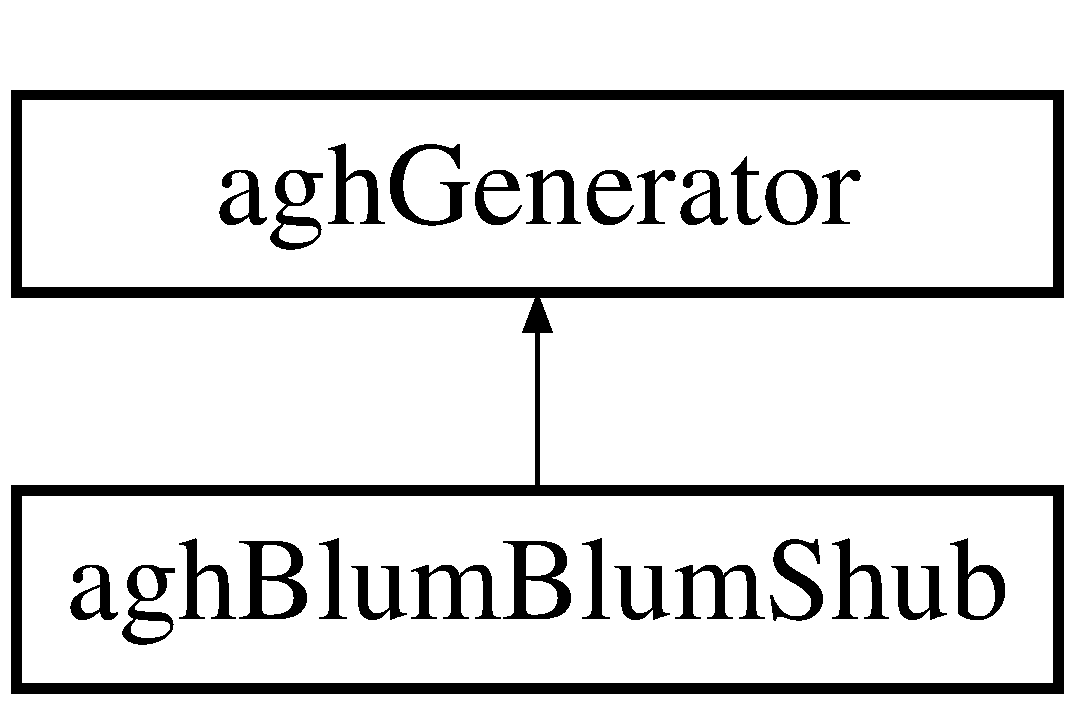
\includegraphics[height=2.000000cm]{classaghBlumBlumShub}
\end{center}
\end{figure}
\subsection*{\-Public \-Member \-Functions}
\begin{DoxyCompactItemize}
\item 
\hypertarget{classaghBlumBlumShub_a9396f651ba093efee9bdbdd6371d468c}{\hyperlink{classaghBlumBlumShub_a9396f651ba093efee9bdbdd6371d468c}{agh\-Blum\-Blum\-Shub} ()}\label{classaghBlumBlumShub_a9396f651ba093efee9bdbdd6371d468c}

\begin{DoxyCompactList}\small\item\em \-Konstruktor bezparametrowy klasy. \end{DoxyCompactList}\item 
\hyperlink{classaghBlumBlumShub_a1188d0744baa38f49c10333021bd864a}{agh\-Blum\-Blum\-Shub} (int \-\_\-poczatek\-Zakres, int \-\_\-koniec\-Zakres, int \-\_\-ziarno, int \-\_\-pierwsza\-P, int \-\_\-pierwsza\-Q)
\begin{DoxyCompactList}\small\item\em \-Konstruktor parametrowy klasy. \end{DoxyCompactList}\item 
virtual void \hyperlink{classaghBlumBlumShub_a5c227b9f3044159544ac20fb5b1f2e1c}{ustaw\-Ziarno} (int \-\_\-ziarno)
\begin{DoxyCompactList}\small\item\em \-Wirtualna funkcja ustawaijąca ziarno. \end{DoxyCompactList}\item 
void \hyperlink{classaghBlumBlumShub_a194c8137ab486ea0a95b56fc4485566f}{ustaw\-Pierwsza\-P} (int \-\_\-pierwsza\-P)
\begin{DoxyCompactList}\small\item\em \-Funkcja ustawaijąca liczbe pierwszą \end{DoxyCompactList}\item 
void \hyperlink{classaghBlumBlumShub_a9b03ee0b06b667acaaec54b81cdefbbe}{ustaw\-Pierwsza\-Q} (int \-\_\-pierwsza\-Q)
\begin{DoxyCompactList}\small\item\em \-Funkcja ustawaijąca liczbe pierwszą \end{DoxyCompactList}\item 
virtual int \hyperlink{classaghBlumBlumShub_a4aacbcc18ec41812820301959857ce29}{losuj\-Liczbe} ()
\begin{DoxyCompactList}\small\item\em \-Wirtualna funkcja losująca liczbę \end{DoxyCompactList}\end{DoxyCompactItemize}


\subsection{\-Detailed \-Description}
\-Definicja klasy \hyperlink{classaghBlumBlumShub}{agh\-Blum\-Blum\-Shub}. 

\begin{DoxyAuthor}{\-Author}
\-Izabela Śmietana \& \-Krzysztof \-Spytkowski 
\end{DoxyAuthor}
\begin{DoxyDate}{\-Date}
16.\-05.\-2013 
\end{DoxyDate}


\subsection{\-Constructor \& \-Destructor \-Documentation}
\hypertarget{classaghBlumBlumShub_a1188d0744baa38f49c10333021bd864a}{\index{agh\-Blum\-Blum\-Shub@{agh\-Blum\-Blum\-Shub}!agh\-Blum\-Blum\-Shub@{agh\-Blum\-Blum\-Shub}}
\index{agh\-Blum\-Blum\-Shub@{agh\-Blum\-Blum\-Shub}!aghBlumBlumShub@{agh\-Blum\-Blum\-Shub}}
\subsubsection[{agh\-Blum\-Blum\-Shub}]{\setlength{\rightskip}{0pt plus 5cm}{\bf agh\-Blum\-Blum\-Shub\-::agh\-Blum\-Blum\-Shub} (
\begin{DoxyParamCaption}
\item[{int}]{\-\_\-poczatek\-Zakres, }
\item[{int}]{\-\_\-koniec\-Zakres, }
\item[{int}]{\-\_\-ziarno, }
\item[{int}]{\-\_\-pierwsza\-P, }
\item[{int}]{\-\_\-pierwsza\-Q}
\end{DoxyParamCaption}
)}}\label{classaghBlumBlumShub_a1188d0744baa38f49c10333021bd864a}


\-Konstruktor parametrowy klasy. 


\begin{DoxyParams}{\-Parameters}
{\em \-\_\-poczatek\-Zakres} & -\/ \-Poczatek zakresu losowanych liczb \\
\hline
{\em \-\_\-koniec\-Zakres} & -\/ \-Koniec zakresu losowanych liczb \\
\hline
{\em \-\_\-ziarno} & -\/ \-Ziarno \\
\hline
{\em \-\_\-pierwsza\-P} & -\/ \-Liczba pierwsza \\
\hline
{\em \-\_\-pierwsza\-Q} & -\/ \-Liczba pierwsza \\
\hline
\end{DoxyParams}


\subsection{\-Member \-Function \-Documentation}
\hypertarget{classaghBlumBlumShub_a4aacbcc18ec41812820301959857ce29}{\index{agh\-Blum\-Blum\-Shub@{agh\-Blum\-Blum\-Shub}!losuj\-Liczbe@{losuj\-Liczbe}}
\index{losuj\-Liczbe@{losuj\-Liczbe}!aghBlumBlumShub@{agh\-Blum\-Blum\-Shub}}
\subsubsection[{losuj\-Liczbe}]{\setlength{\rightskip}{0pt plus 5cm}int {\bf agh\-Blum\-Blum\-Shub\-::losuj\-Liczbe} (
\begin{DoxyParamCaption}
{}
\end{DoxyParamCaption}
)\hspace{0.3cm}{\ttfamily  \mbox{[}virtual\mbox{]}}}}\label{classaghBlumBlumShub_a4aacbcc18ec41812820301959857ce29}


\-Wirtualna funkcja losująca liczbę 

\begin{DoxyReturn}{\-Returns}
\-Wylosowana liczba 
\end{DoxyReturn}


\-Implements \hyperlink{classaghGenerator_ae0f3bbfe8a7d233c006728c060a2e453}{agh\-Generator}.

\hypertarget{classaghBlumBlumShub_a194c8137ab486ea0a95b56fc4485566f}{\index{agh\-Blum\-Blum\-Shub@{agh\-Blum\-Blum\-Shub}!ustaw\-Pierwsza\-P@{ustaw\-Pierwsza\-P}}
\index{ustaw\-Pierwsza\-P@{ustaw\-Pierwsza\-P}!aghBlumBlumShub@{agh\-Blum\-Blum\-Shub}}
\subsubsection[{ustaw\-Pierwsza\-P}]{\setlength{\rightskip}{0pt plus 5cm}void {\bf agh\-Blum\-Blum\-Shub\-::ustaw\-Pierwsza\-P} (
\begin{DoxyParamCaption}
\item[{int}]{\-\_\-pierwsza\-P}
\end{DoxyParamCaption}
)}}\label{classaghBlumBlumShub_a194c8137ab486ea0a95b56fc4485566f}


\-Funkcja ustawaijąca liczbe pierwszą 


\begin{DoxyParams}{\-Parameters}
{\em \-\_\-pierwsza\-P} & -\/ \-Liczba pierwsza \\
\hline
\end{DoxyParams}
\hypertarget{classaghBlumBlumShub_a9b03ee0b06b667acaaec54b81cdefbbe}{\index{agh\-Blum\-Blum\-Shub@{agh\-Blum\-Blum\-Shub}!ustaw\-Pierwsza\-Q@{ustaw\-Pierwsza\-Q}}
\index{ustaw\-Pierwsza\-Q@{ustaw\-Pierwsza\-Q}!aghBlumBlumShub@{agh\-Blum\-Blum\-Shub}}
\subsubsection[{ustaw\-Pierwsza\-Q}]{\setlength{\rightskip}{0pt plus 5cm}void {\bf agh\-Blum\-Blum\-Shub\-::ustaw\-Pierwsza\-Q} (
\begin{DoxyParamCaption}
\item[{int}]{\-\_\-pierwsza\-Q}
\end{DoxyParamCaption}
)}}\label{classaghBlumBlumShub_a9b03ee0b06b667acaaec54b81cdefbbe}


\-Funkcja ustawaijąca liczbe pierwszą 


\begin{DoxyParams}{\-Parameters}
{\em \-\_\-pierwsza\-Q} & -\/ \-Liczba pierwsza \\
\hline
\end{DoxyParams}
\hypertarget{classaghBlumBlumShub_a5c227b9f3044159544ac20fb5b1f2e1c}{\index{agh\-Blum\-Blum\-Shub@{agh\-Blum\-Blum\-Shub}!ustaw\-Ziarno@{ustaw\-Ziarno}}
\index{ustaw\-Ziarno@{ustaw\-Ziarno}!aghBlumBlumShub@{agh\-Blum\-Blum\-Shub}}
\subsubsection[{ustaw\-Ziarno}]{\setlength{\rightskip}{0pt plus 5cm}void {\bf agh\-Blum\-Blum\-Shub\-::ustaw\-Ziarno} (
\begin{DoxyParamCaption}
\item[{int}]{\-\_\-ziarno}
\end{DoxyParamCaption}
)\hspace{0.3cm}{\ttfamily  \mbox{[}virtual\mbox{]}}}}\label{classaghBlumBlumShub_a5c227b9f3044159544ac20fb5b1f2e1c}


\-Wirtualna funkcja ustawaijąca ziarno. 


\begin{DoxyParams}{\-Parameters}
{\em \-\_\-ziarno} & -\/ \-Ziarno \\
\hline
\end{DoxyParams}


\-Reimplemented from \hyperlink{classaghGenerator_aeb8309c8c8d14bb1df9a594776399a23}{agh\-Generator}.



\-The documentation for this class was generated from the following files\-:\begin{DoxyCompactItemize}
\item 
\hyperlink{aghBlumBlumShub_8h}{agh\-Blum\-Blum\-Shub.\-h}\item 
agh\-Blum\-Blum\-Shub.\-cpp\end{DoxyCompactItemize}

\hypertarget{classaghChiKwadrat}{\section{agh\-Chi\-Kwadrat \-Class \-Reference}
\label{classaghChiKwadrat}\index{agh\-Chi\-Kwadrat@{agh\-Chi\-Kwadrat}}
}


\-Definicja klasy \hyperlink{classaghChiKwadrat}{agh\-Chi\-Kwadrat}.  




{\ttfamily \#include $<$agh\-Chi\-Kwadrat.\-h$>$}

\-Inheritance diagram for agh\-Chi\-Kwadrat\-:\begin{figure}[H]
\begin{center}
\leavevmode
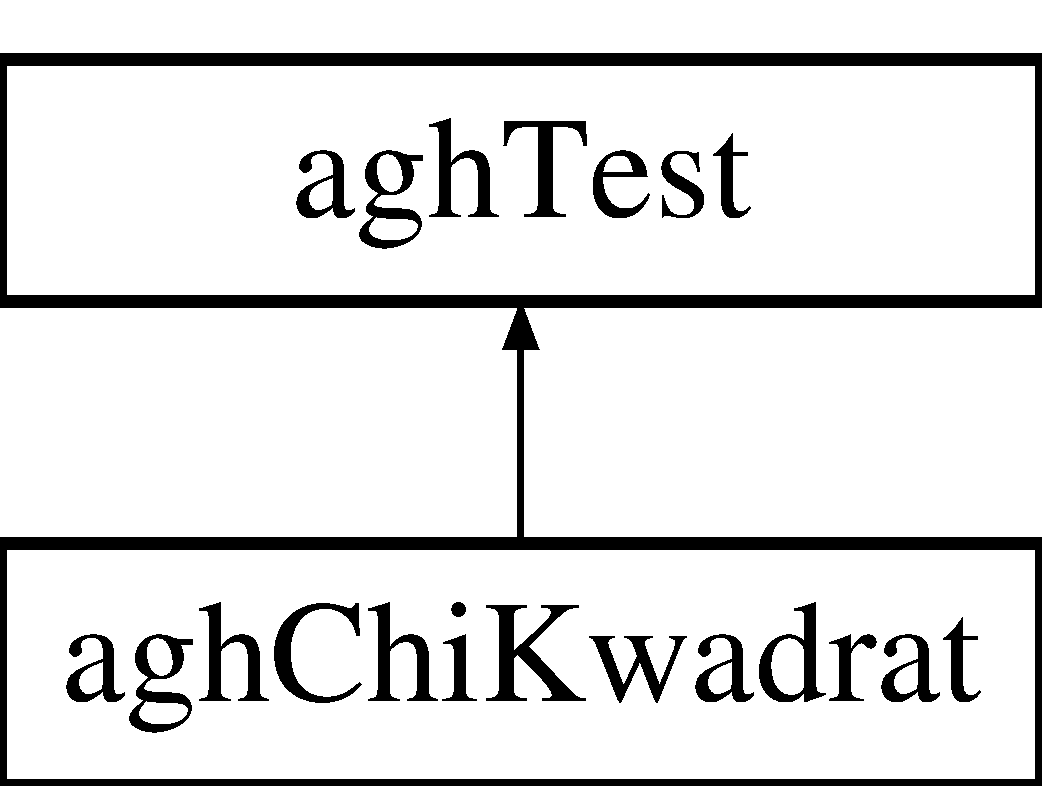
\includegraphics[height=2.000000cm]{classaghChiKwadrat}
\end{center}
\end{figure}
\subsection*{\-Public \-Member \-Functions}
\begin{DoxyCompactItemize}
\item 
\hypertarget{classaghChiKwadrat_a82ef352017c05e8a111a19200525c65e}{\hyperlink{classaghChiKwadrat_a82ef352017c05e8a111a19200525c65e}{agh\-Chi\-Kwadrat} ()}\label{classaghChiKwadrat_a82ef352017c05e8a111a19200525c65e}

\begin{DoxyCompactList}\small\item\em \-Konstruktor bezparametrowy klasy. \end{DoxyCompactList}\item 
\hyperlink{classaghChiKwadrat_ac0f7804068dddd48a41a6045bba597c2}{agh\-Chi\-Kwadrat} (\hyperlink{classaghGenerator}{agh\-Generator} $\ast$\-\_\-wsk\-Generator, int \-\_\-ilosc\-Liczb, int \-\_\-liczba\-Przedzialow)
\begin{DoxyCompactList}\small\item\em \-Konstruktor parametrowy klasy. \end{DoxyCompactList}\item 
\hypertarget{classaghChiKwadrat_a8246e5e80c1bbed7c68b33c9e3a432dc}{void \hyperlink{classaghChiKwadrat_a8246e5e80c1bbed7c68b33c9e3a432dc}{ustaw\-Liczba\-Przedzialow} (int \-\_\-liczba\-Przedzialow)}\label{classaghChiKwadrat_a8246e5e80c1bbed7c68b33c9e3a432dc}

\begin{DoxyCompactList}\small\item\em \-Funkcja ustawiająca liczbę przedzialow. \end{DoxyCompactList}\item 
\hypertarget{classaghChiKwadrat_a533a052340dae56d6209093cc8c7365e}{virtual void \hyperlink{classaghChiKwadrat_a533a052340dae56d6209093cc8c7365e}{testuj} ()}\label{classaghChiKwadrat_a533a052340dae56d6209093cc8c7365e}

\begin{DoxyCompactList}\small\item\em \-Wirtualna funkcja testująca generator. \end{DoxyCompactList}\item 
virtual void \hyperlink{classaghChiKwadrat_a6d86b271437ada0f232164812a3671c5}{wypisz} (ostream \&strumien=cout)
\begin{DoxyCompactList}\small\item\em \-Wirtualna funkcja wypisująca na zadany strumien wynik testu. \end{DoxyCompactList}\end{DoxyCompactItemize}


\subsection{\-Detailed \-Description}
\-Definicja klasy \hyperlink{classaghChiKwadrat}{agh\-Chi\-Kwadrat}. 

\begin{DoxyAuthor}{\-Author}
\-Izabela Śmietana \& \-Krzysztof \-Spytkowski 
\end{DoxyAuthor}
\begin{DoxyDate}{\-Date}
16.\-05.\-2013 
\end{DoxyDate}


\subsection{\-Constructor \& \-Destructor \-Documentation}
\hypertarget{classaghChiKwadrat_ac0f7804068dddd48a41a6045bba597c2}{\index{agh\-Chi\-Kwadrat@{agh\-Chi\-Kwadrat}!agh\-Chi\-Kwadrat@{agh\-Chi\-Kwadrat}}
\index{agh\-Chi\-Kwadrat@{agh\-Chi\-Kwadrat}!aghChiKwadrat@{agh\-Chi\-Kwadrat}}
\subsubsection[{agh\-Chi\-Kwadrat}]{\setlength{\rightskip}{0pt plus 5cm}{\bf agh\-Chi\-Kwadrat\-::agh\-Chi\-Kwadrat} (
\begin{DoxyParamCaption}
\item[{{\bf agh\-Generator} $\ast$}]{\-\_\-wsk\-Generator, }
\item[{int}]{\-\_\-ilosc\-Liczb, }
\item[{int}]{\-\_\-liczba\-Przedzialow}
\end{DoxyParamCaption}
)}}\label{classaghChiKwadrat_ac0f7804068dddd48a41a6045bba597c2}


\-Konstruktor parametrowy klasy. 


\begin{DoxyParams}{\-Parameters}
{\em \-\_\-wsk\-Generator} & -\/ \-Wskaźnik na generator \\
\hline
{\em \-\_\-ilosc\-Liczb} & -\/ \-Ilośc liczb do wylosowania \\
\hline
{\em \-\_\-liczba\-Przedzialow} & -\/ \-Liczba przedzialow \\
\hline
\end{DoxyParams}


\subsection{\-Member \-Function \-Documentation}
\hypertarget{classaghChiKwadrat_a6d86b271437ada0f232164812a3671c5}{\index{agh\-Chi\-Kwadrat@{agh\-Chi\-Kwadrat}!wypisz@{wypisz}}
\index{wypisz@{wypisz}!aghChiKwadrat@{agh\-Chi\-Kwadrat}}
\subsubsection[{wypisz}]{\setlength{\rightskip}{0pt plus 5cm}void {\bf agh\-Chi\-Kwadrat\-::wypisz} (
\begin{DoxyParamCaption}
\item[{ostream \&}]{strumien = {\ttfamily cout}}
\end{DoxyParamCaption}
)\hspace{0.3cm}{\ttfamily  \mbox{[}virtual\mbox{]}}}}\label{classaghChiKwadrat_a6d86b271437ada0f232164812a3671c5}


\-Wirtualna funkcja wypisująca na zadany strumien wynik testu. 


\begin{DoxyParams}{\-Parameters}
{\em strumien} & -\/ \-Strumien, na który należy wypisać wynik testu (domyślnie cout) \\
\hline
\end{DoxyParams}


\-Implements \hyperlink{classaghTest_ad43c3c9a98d652936d9a5fe90aa1b57b}{agh\-Test}.



\-The documentation for this class was generated from the following files\-:\begin{DoxyCompactItemize}
\item 
\hyperlink{aghChiKwadrat_8h}{agh\-Chi\-Kwadrat.\-h}\item 
agh\-Chi\-Kwadrat.\-cpp\end{DoxyCompactItemize}

\hypertarget{classaghException}{\section{agh\-Exception \-Class \-Reference}
\label{classaghException}\index{agh\-Exception@{agh\-Exception}}
}


\-The definition of \hyperlink{classaghException}{agh\-Exception} class that allows for exception handling.  




{\ttfamily \#include $<$agh\-Exception.\-h$>$}

\subsection*{\-Public \-Member \-Functions}
\begin{DoxyCompactItemize}
\item 
\hypertarget{classaghException_a4823634f8bfb0fe7338b49f0e26fc90a}{\hyperlink{classaghException_a4823634f8bfb0fe7338b49f0e26fc90a}{agh\-Exception} (void)}\label{classaghException_a4823634f8bfb0fe7338b49f0e26fc90a}

\begin{DoxyCompactList}\small\item\em \-The default constructor. \end{DoxyCompactList}\item 
\hyperlink{classaghException_aab9f50f92dd98ed21ada6640b5c08c35}{agh\-Exception} (\hyperlink{classaghException}{agh\-Exception} const \&\-\_\-\-\_\-other)
\begin{DoxyCompactList}\small\item\em \-The copying constructor. \end{DoxyCompactList}\item 
\hyperlink{classaghException_a477a774d6e9f879d019fafa73991080a}{agh\-Exception} (int \-\_\-\-\_\-error\-Code, int \-\_\-\-\_\-error\-Line)
\begin{DoxyCompactList}\small\item\em \-The class contructor. \end{DoxyCompactList}\item 
\hyperlink{classaghException_a6b160541a62b35ed167464925ff65cee}{agh\-Exception} (int \-\_\-\-\_\-error\-Code, string \-\_\-\-\_\-error\-Message)
\begin{DoxyCompactList}\small\item\em \-The class contructor. \end{DoxyCompactList}\item 
\hyperlink{classaghException_abd29488d2def0dac2fe1dfc5f3737e4b}{agh\-Exception} (string \-\_\-\-\_\-error\-File, int \-\_\-\-\_\-error\-Line)
\begin{DoxyCompactList}\small\item\em \-The class constructor. \end{DoxyCompactList}\item 
\hyperlink{classaghException_aa77df63b302cc2829178f49fa7f9aa53}{agh\-Exception} (int \-\_\-\-\_\-error\-Code, string \-\_\-\-\_\-error\-Message, string \-\_\-\-\_\-error\-File, int \-\_\-\-\_\-error\-Line)
\begin{DoxyCompactList}\small\item\em \-The class constructor. \end{DoxyCompactList}\item 
\hypertarget{classaghException_acdf702b31955bd115042a8c22fdde3b0}{virtual \hyperlink{classaghException_acdf702b31955bd115042a8c22fdde3b0}{$\sim$agh\-Exception} (void)}\label{classaghException_acdf702b31955bd115042a8c22fdde3b0}

\begin{DoxyCompactList}\small\item\em \-The class destructor. \end{DoxyCompactList}\item 
virtual int \hyperlink{classaghException_aa6e25c04b7ceed6fbb5ca9b3c780921b}{error\-Code} (void) const 
\begin{DoxyCompactList}\small\item\em \-Virtual function that returns the error code. \end{DoxyCompactList}\item 
virtual int \hyperlink{classaghException_aecaea0d8a8a6f5740fbeb393e0d1c2e8}{error\-Line} (void) const 
\begin{DoxyCompactList}\small\item\em \-Virtual function that returns the line in the file where the error occured. \end{DoxyCompactList}\item 
virtual string \hyperlink{classaghException_acd71f90fa8decaceebc110e61bc11e26}{error\-Message} (void) const 
\begin{DoxyCompactList}\small\item\em \-Virtual function that returns the error message for a user. \end{DoxyCompactList}\item 
virtual string \hyperlink{classaghException_a1f5d681faec44b25a1ce5afabe73b9cd}{error\-File} (void) const 
\begin{DoxyCompactList}\small\item\em \-Virtual function that returns the error file name. \end{DoxyCompactList}\item 
virtual void \hyperlink{classaghException_ae181a4bf4fddee1bf470c3079c74deef}{set\-Error\-Line} (int \-\_\-\-\_\-error\-Line)
\begin{DoxyCompactList}\small\item\em \-Virtual function that sets the error line number. \end{DoxyCompactList}\item 
virtual void \hyperlink{classaghException_a6d415efebe645970a3eac339a33b5aa9}{set\-Error\-Code} (int \-\_\-\-\_\-error\-Code)
\begin{DoxyCompactList}\small\item\em \-Virtual function that sets the error code. \end{DoxyCompactList}\item 
virtual void \hyperlink{classaghException_a3b89888678fa5d33827386d2ed9d8d3a}{set\-Error\-Message} (string \-\_\-\-\_\-error\-Message)
\begin{DoxyCompactList}\small\item\em \-Virtual function that sets the error message. \end{DoxyCompactList}\item 
virtual void \hyperlink{classaghException_a94b807f0f954e4ff09bdcb104f7388f4}{set\-Error\-File} (string \-\_\-\-\_\-error\-File)
\begin{DoxyCompactList}\small\item\em \-Virtual function that sets the error file name. \end{DoxyCompactList}\item 
\hyperlink{classaghException}{agh\-Exception} \& \hyperlink{classaghException_a648edf43a073c5141bf1cd7079b61230}{operator=} (\hyperlink{classaghException}{agh\-Exception} const \&\-\_\-\-\_\-other)
\begin{DoxyCompactList}\small\item\em \-Assigments operator. \end{DoxyCompactList}\end{DoxyCompactItemize}


\subsection{\-Detailed \-Description}
\-The definition of \hyperlink{classaghException}{agh\-Exception} class that allows for exception handling. 

\begin{DoxyAuthor}{\-Author}
\-Krzysztof \-Kaczor 
\end{DoxyAuthor}
\begin{DoxyDate}{\-Date}
15.\-04.\-2011 
\end{DoxyDate}


\subsection{\-Constructor \& \-Destructor \-Documentation}
\hypertarget{classaghException_aab9f50f92dd98ed21ada6640b5c08c35}{\index{agh\-Exception@{agh\-Exception}!agh\-Exception@{agh\-Exception}}
\index{agh\-Exception@{agh\-Exception}!aghException@{agh\-Exception}}
\subsubsection[{agh\-Exception}]{\setlength{\rightskip}{0pt plus 5cm}{\bf agh\-Exception\-::agh\-Exception} (
\begin{DoxyParamCaption}
\item[{{\bf agh\-Exception} const \&}]{\-\_\-\-\_\-other}
\end{DoxyParamCaption}
)}}\label{classaghException_aab9f50f92dd98ed21ada6640b5c08c35}


\-The copying constructor. 


\begin{DoxyParams}{\-Parameters}
{\em \-\_\-\-\_\-other} & -\/ the source object \\
\hline
\end{DoxyParams}
\hypertarget{classaghException_a477a774d6e9f879d019fafa73991080a}{\index{agh\-Exception@{agh\-Exception}!agh\-Exception@{agh\-Exception}}
\index{agh\-Exception@{agh\-Exception}!aghException@{agh\-Exception}}
\subsubsection[{agh\-Exception}]{\setlength{\rightskip}{0pt plus 5cm}{\bf agh\-Exception\-::agh\-Exception} (
\begin{DoxyParamCaption}
\item[{int}]{\-\_\-\-\_\-error\-Code, }
\item[{int}]{\-\_\-\-\_\-error\-Line}
\end{DoxyParamCaption}
)}}\label{classaghException_a477a774d6e9f879d019fafa73991080a}


\-The class contructor. 


\begin{DoxyParams}{\-Parameters}
{\em \-\_\-\-\_\-error\-Code} & -\/ code of the error \\
\hline
{\em \-\_\-\-\_\-error\-Line} & -\/ line (in the file) where the error occured \\
\hline
\end{DoxyParams}
\hypertarget{classaghException_a6b160541a62b35ed167464925ff65cee}{\index{agh\-Exception@{agh\-Exception}!agh\-Exception@{agh\-Exception}}
\index{agh\-Exception@{agh\-Exception}!aghException@{agh\-Exception}}
\subsubsection[{agh\-Exception}]{\setlength{\rightskip}{0pt plus 5cm}{\bf agh\-Exception\-::agh\-Exception} (
\begin{DoxyParamCaption}
\item[{int}]{\-\_\-\-\_\-error\-Code, }
\item[{string}]{\-\_\-\-\_\-error\-Message}
\end{DoxyParamCaption}
)}}\label{classaghException_a6b160541a62b35ed167464925ff65cee}


\-The class contructor. 


\begin{DoxyParams}{\-Parameters}
{\em \-\_\-\-\_\-error\-Code} & -\/ code of the error \\
\hline
{\em \-\_\-\-\_\-error\-Message} & -\/ the error message for the user \\
\hline
\end{DoxyParams}
\hypertarget{classaghException_abd29488d2def0dac2fe1dfc5f3737e4b}{\index{agh\-Exception@{agh\-Exception}!agh\-Exception@{agh\-Exception}}
\index{agh\-Exception@{agh\-Exception}!aghException@{agh\-Exception}}
\subsubsection[{agh\-Exception}]{\setlength{\rightskip}{0pt plus 5cm}{\bf agh\-Exception\-::agh\-Exception} (
\begin{DoxyParamCaption}
\item[{string}]{\-\_\-\-\_\-error\-File, }
\item[{int}]{\-\_\-\-\_\-error\-Line}
\end{DoxyParamCaption}
)}}\label{classaghException_abd29488d2def0dac2fe1dfc5f3737e4b}


\-The class constructor. 


\begin{DoxyParams}{\-Parameters}
{\em \-\_\-\-\_\-error\-File} & -\/ the name of the file where the error occured \\
\hline
{\em \-\_\-\-\_\-error\-Line} & -\/ the line in the file where the error occured \\
\hline
\end{DoxyParams}
\hypertarget{classaghException_aa77df63b302cc2829178f49fa7f9aa53}{\index{agh\-Exception@{agh\-Exception}!agh\-Exception@{agh\-Exception}}
\index{agh\-Exception@{agh\-Exception}!aghException@{agh\-Exception}}
\subsubsection[{agh\-Exception}]{\setlength{\rightskip}{0pt plus 5cm}{\bf agh\-Exception\-::agh\-Exception} (
\begin{DoxyParamCaption}
\item[{int}]{\-\_\-\-\_\-error\-Code, }
\item[{string}]{\-\_\-\-\_\-error\-Message, }
\item[{string}]{\-\_\-\-\_\-error\-File, }
\item[{int}]{\-\_\-\-\_\-error\-Line}
\end{DoxyParamCaption}
)}}\label{classaghException_aa77df63b302cc2829178f49fa7f9aa53}


\-The class constructor. 


\begin{DoxyParams}{\-Parameters}
{\em \-\_\-\-\_\-error\-Code} & -\/ code of the error \\
\hline
{\em \-\_\-\-\_\-error\-Message} & -\/ the error message for the user \\
\hline
{\em \-\_\-\-\_\-error\-File} & -\/ the name of the file where the error occured \\
\hline
{\em \-\_\-\-\_\-error\-Line} & -\/ the line in the file where the error occured \\
\hline
\end{DoxyParams}


\subsection{\-Member \-Function \-Documentation}
\hypertarget{classaghException_aa6e25c04b7ceed6fbb5ca9b3c780921b}{\index{agh\-Exception@{agh\-Exception}!error\-Code@{error\-Code}}
\index{error\-Code@{error\-Code}!aghException@{agh\-Exception}}
\subsubsection[{error\-Code}]{\setlength{\rightskip}{0pt plus 5cm}int {\bf agh\-Exception\-::error\-Code} (
\begin{DoxyParamCaption}
\item[{void}]{}
\end{DoxyParamCaption}
) const\hspace{0.3cm}{\ttfamily  \mbox{[}virtual\mbox{]}}}}\label{classaghException_aa6e25c04b7ceed6fbb5ca9b3c780921b}


\-Virtual function that returns the error code. 

\begin{DoxyReturn}{\-Returns}
a value of the \-\_\-error\-Code field 
\end{DoxyReturn}
\hypertarget{classaghException_a1f5d681faec44b25a1ce5afabe73b9cd}{\index{agh\-Exception@{agh\-Exception}!error\-File@{error\-File}}
\index{error\-File@{error\-File}!aghException@{agh\-Exception}}
\subsubsection[{error\-File}]{\setlength{\rightskip}{0pt plus 5cm}string {\bf agh\-Exception\-::error\-File} (
\begin{DoxyParamCaption}
\item[{void}]{}
\end{DoxyParamCaption}
) const\hspace{0.3cm}{\ttfamily  \mbox{[}virtual\mbox{]}}}}\label{classaghException_a1f5d681faec44b25a1ce5afabe73b9cd}


\-Virtual function that returns the error file name. 

\begin{DoxyReturn}{\-Returns}
a value of the \-\_\-error\-File field 
\end{DoxyReturn}
\hypertarget{classaghException_aecaea0d8a8a6f5740fbeb393e0d1c2e8}{\index{agh\-Exception@{agh\-Exception}!error\-Line@{error\-Line}}
\index{error\-Line@{error\-Line}!aghException@{agh\-Exception}}
\subsubsection[{error\-Line}]{\setlength{\rightskip}{0pt plus 5cm}int {\bf agh\-Exception\-::error\-Line} (
\begin{DoxyParamCaption}
\item[{void}]{}
\end{DoxyParamCaption}
) const\hspace{0.3cm}{\ttfamily  \mbox{[}virtual\mbox{]}}}}\label{classaghException_aecaea0d8a8a6f5740fbeb393e0d1c2e8}


\-Virtual function that returns the line in the file where the error occured. 

\begin{DoxyReturn}{\-Returns}
a value of the \-\_\-error\-Line field 
\end{DoxyReturn}
\hypertarget{classaghException_acd71f90fa8decaceebc110e61bc11e26}{\index{agh\-Exception@{agh\-Exception}!error\-Message@{error\-Message}}
\index{error\-Message@{error\-Message}!aghException@{agh\-Exception}}
\subsubsection[{error\-Message}]{\setlength{\rightskip}{0pt plus 5cm}string {\bf agh\-Exception\-::error\-Message} (
\begin{DoxyParamCaption}
\item[{void}]{}
\end{DoxyParamCaption}
) const\hspace{0.3cm}{\ttfamily  \mbox{[}virtual\mbox{]}}}}\label{classaghException_acd71f90fa8decaceebc110e61bc11e26}


\-Virtual function that returns the error message for a user. 

\begin{DoxyReturn}{\-Returns}
a value of the \-\_\-error\-Message field 
\end{DoxyReturn}
\hypertarget{classaghException_a648edf43a073c5141bf1cd7079b61230}{\index{agh\-Exception@{agh\-Exception}!operator=@{operator=}}
\index{operator=@{operator=}!aghException@{agh\-Exception}}
\subsubsection[{operator=}]{\setlength{\rightskip}{0pt plus 5cm}{\bf agh\-Exception} \& agh\-Exception\-::operator= (
\begin{DoxyParamCaption}
\item[{{\bf agh\-Exception} const \&}]{\-\_\-\-\_\-other}
\end{DoxyParamCaption}
)}}\label{classaghException_a648edf43a073c5141bf1cd7079b61230}


\-Assigments operator. 


\begin{DoxyParams}{\-Parameters}
{\em \-\_\-\-\_\-other} & -\/ the source object \\
\hline
\end{DoxyParams}
\begin{DoxyReturn}{\-Returns}
reference to this object 
\end{DoxyReturn}
\hypertarget{classaghException_a6d415efebe645970a3eac339a33b5aa9}{\index{agh\-Exception@{agh\-Exception}!set\-Error\-Code@{set\-Error\-Code}}
\index{set\-Error\-Code@{set\-Error\-Code}!aghException@{agh\-Exception}}
\subsubsection[{set\-Error\-Code}]{\setlength{\rightskip}{0pt plus 5cm}void {\bf agh\-Exception\-::set\-Error\-Code} (
\begin{DoxyParamCaption}
\item[{int}]{\-\_\-\-\_\-error\-Code}
\end{DoxyParamCaption}
)\hspace{0.3cm}{\ttfamily  \mbox{[}virtual\mbox{]}}}}\label{classaghException_a6d415efebe645970a3eac339a33b5aa9}


\-Virtual function that sets the error code. 


\begin{DoxyParams}{\-Parameters}
{\em \-\_\-\-\_\-error\-Code} & -\/ a new value of the \-\_\-error\-Code field \\
\hline
\end{DoxyParams}
\begin{DoxyReturn}{\-Returns}
no values return 
\end{DoxyReturn}
\hypertarget{classaghException_a94b807f0f954e4ff09bdcb104f7388f4}{\index{agh\-Exception@{agh\-Exception}!set\-Error\-File@{set\-Error\-File}}
\index{set\-Error\-File@{set\-Error\-File}!aghException@{agh\-Exception}}
\subsubsection[{set\-Error\-File}]{\setlength{\rightskip}{0pt plus 5cm}void {\bf agh\-Exception\-::set\-Error\-File} (
\begin{DoxyParamCaption}
\item[{string}]{\-\_\-\-\_\-error\-File}
\end{DoxyParamCaption}
)\hspace{0.3cm}{\ttfamily  \mbox{[}virtual\mbox{]}}}}\label{classaghException_a94b807f0f954e4ff09bdcb104f7388f4}


\-Virtual function that sets the error file name. 


\begin{DoxyParams}{\-Parameters}
{\em \-\_\-\-\_\-error\-File} & -\/ a new value of the \-\_\-error\-File field \\
\hline
\end{DoxyParams}
\begin{DoxyReturn}{\-Returns}
no values return 
\end{DoxyReturn}
\hypertarget{classaghException_ae181a4bf4fddee1bf470c3079c74deef}{\index{agh\-Exception@{agh\-Exception}!set\-Error\-Line@{set\-Error\-Line}}
\index{set\-Error\-Line@{set\-Error\-Line}!aghException@{agh\-Exception}}
\subsubsection[{set\-Error\-Line}]{\setlength{\rightskip}{0pt plus 5cm}void {\bf agh\-Exception\-::set\-Error\-Line} (
\begin{DoxyParamCaption}
\item[{int}]{\-\_\-\-\_\-error\-Line}
\end{DoxyParamCaption}
)\hspace{0.3cm}{\ttfamily  \mbox{[}virtual\mbox{]}}}}\label{classaghException_ae181a4bf4fddee1bf470c3079c74deef}


\-Virtual function that sets the error line number. 


\begin{DoxyParams}{\-Parameters}
{\em \-\_\-\-\_\-error\-Line} & -\/ a new value of the \-\_\-error\-Line field \\
\hline
\end{DoxyParams}
\begin{DoxyReturn}{\-Returns}
no values return 
\end{DoxyReturn}
\hypertarget{classaghException_a3b89888678fa5d33827386d2ed9d8d3a}{\index{agh\-Exception@{agh\-Exception}!set\-Error\-Message@{set\-Error\-Message}}
\index{set\-Error\-Message@{set\-Error\-Message}!aghException@{agh\-Exception}}
\subsubsection[{set\-Error\-Message}]{\setlength{\rightskip}{0pt plus 5cm}void {\bf agh\-Exception\-::set\-Error\-Message} (
\begin{DoxyParamCaption}
\item[{string}]{\-\_\-\-\_\-error\-Message}
\end{DoxyParamCaption}
)\hspace{0.3cm}{\ttfamily  \mbox{[}virtual\mbox{]}}}}\label{classaghException_a3b89888678fa5d33827386d2ed9d8d3a}


\-Virtual function that sets the error message. 


\begin{DoxyParams}{\-Parameters}
{\em \-\_\-\-\_\-error\-Message} & -\/ a new value of the \-\_\-error\-Message field \\
\hline
\end{DoxyParams}
\begin{DoxyReturn}{\-Returns}
no values return 
\end{DoxyReturn}


\-The documentation for this class was generated from the following files\-:\begin{DoxyCompactItemize}
\item 
\hyperlink{aghException_8h}{agh\-Exception.\-h}\item 
agh\-Exception.\-cpp\end{DoxyCompactItemize}

\hypertarget{classaghGenerator}{\section{agh\-Generator \-Class \-Reference}
\label{classaghGenerator}\index{agh\-Generator@{agh\-Generator}}
}


\-Definicja klasy abstrakcyjnej \hyperlink{classaghGenerator}{agh\-Generator}.  




{\ttfamily \#include $<$agh\-Generator.\-h$>$}

\-Inheritance diagram for agh\-Generator\-:\begin{figure}[H]
\begin{center}
\leavevmode
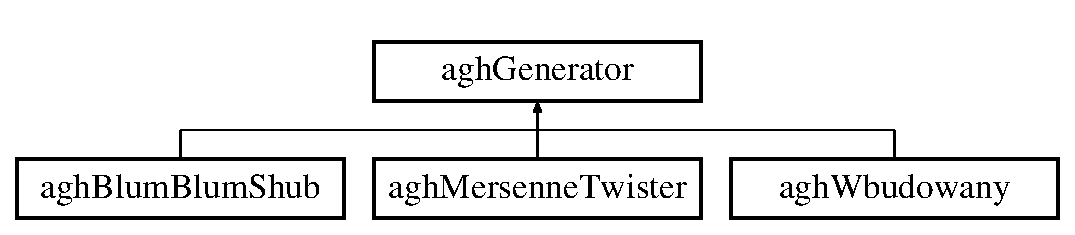
\includegraphics[height=2.000000cm]{classaghGenerator}
\end{center}
\end{figure}
\subsection*{\-Public \-Member \-Functions}
\begin{DoxyCompactItemize}
\item 
\hypertarget{classaghGenerator_a1c8a018e7ad4193ee039187236c0b6f5}{\hyperlink{classaghGenerator_a1c8a018e7ad4193ee039187236c0b6f5}{agh\-Generator} ()}\label{classaghGenerator_a1c8a018e7ad4193ee039187236c0b6f5}

\begin{DoxyCompactList}\small\item\em \-Konstruktor bezparametrowy klasy. \end{DoxyCompactList}\item 
\hyperlink{classaghGenerator_a069ae40df247e8148cdfa50f48fdc73f}{agh\-Generator} (int \-\_\-poczatek\-Zakres, int \-\_\-koniec\-Zakres, int \-\_\-ziarno)
\begin{DoxyCompactList}\small\item\em \-Konstruktor parametrowy klasy. \end{DoxyCompactList}\item 
\hypertarget{classaghGenerator_a65f76f90a98b2bd4a7e4fe57281e71ca}{virtual \hyperlink{classaghGenerator_a65f76f90a98b2bd4a7e4fe57281e71ca}{$\sim$agh\-Generator} ()}\label{classaghGenerator_a65f76f90a98b2bd4a7e4fe57281e71ca}

\begin{DoxyCompactList}\small\item\em \-Wirtualny destruktor klasy. \end{DoxyCompactList}\item 
void \hyperlink{classaghGenerator_a50c965afc1256e0ccb081139b28d546c}{ustaw\-Poczatek} (int \-\_\-poczatek\-Zakres)
\begin{DoxyCompactList}\small\item\em \-Funkcja ustawaijąca poczatek zakresu losowanych liczb. \end{DoxyCompactList}\item 
void \hyperlink{classaghGenerator_ad6417d51d8ff880270cc056efcd6f00c}{ustaw\-Koniec} (int \-\_\-koniec\-Zakres)
\begin{DoxyCompactList}\small\item\em \-Funkcja ustawaijąca koniec zakresu losowanych liczb. \end{DoxyCompactList}\item 
virtual void \hyperlink{classaghGenerator_aeb8309c8c8d14bb1df9a594776399a23}{ustaw\-Ziarno} (int \-\_\-ziarno)
\begin{DoxyCompactList}\small\item\em \-Wirtualna funkcja ustawaijąca ziarno. \end{DoxyCompactList}\item 
int \hyperlink{classaghGenerator_a4c07b2301d4f71f8b2956e9fc79cd3df}{wez\-Poczatek} ()
\begin{DoxyCompactList}\small\item\em \-Funkcja zwracająca poczatek zakresu losowanych liczb. \end{DoxyCompactList}\item 
int \hyperlink{classaghGenerator_aa418dbf03ba3f46b914258eaf5b23b7a}{wez\-Koniec} ()
\begin{DoxyCompactList}\small\item\em \-Funkcja zwracająca koniec zakresu losowanych liczb. \end{DoxyCompactList}\item 
int \hyperlink{classaghGenerator_abaa15dfd5d547a6d64b63153bd2ea765}{wez\-Ziarno} ()
\begin{DoxyCompactList}\small\item\em \-Funkcja zwracająca \-Ziarno. \end{DoxyCompactList}\item 
virtual int \hyperlink{classaghGenerator_ae0f3bbfe8a7d233c006728c060a2e453}{losuj\-Liczbe} ()=0
\begin{DoxyCompactList}\small\item\em \-Czysto wirtualna funkcja losująca liczbę \end{DoxyCompactList}\item 
virtual void \hyperlink{classaghGenerator_a0b082ee64f661bddeabd332a4cd77d4d}{wypisz\-Nazwe} (ostream \&strumien=cout)
\begin{DoxyCompactList}\small\item\em \-Wirtualna funkcja wypisująca na zadany strumien nazwe generatora. \end{DoxyCompactList}\item 
virtual void \hyperlink{classaghGenerator_aa8924c92e6ba31c7e86d0497acf2c7e6}{wypisz\-Liczbe} (ostream \&strumien=cout)
\begin{DoxyCompactList}\small\item\em \-Wirtualna funkcja wypisująca na zadany strumien wylosowaną liczbę \end{DoxyCompactList}\end{DoxyCompactItemize}
\subsection*{\-Protected \-Attributes}
\begin{DoxyCompactItemize}
\item 
\hypertarget{classaghGenerator_acc20585e122620d3516e8562d728f395}{int \hyperlink{classaghGenerator_acc20585e122620d3516e8562d728f395}{poczatek\-Zakres}}\label{classaghGenerator_acc20585e122620d3516e8562d728f395}

\begin{DoxyCompactList}\small\item\em \-Poczatek zakresu losowanych liczb. \end{DoxyCompactList}\item 
\hypertarget{classaghGenerator_a84c85c5027026faba75b363ab47f6d3b}{int \hyperlink{classaghGenerator_a84c85c5027026faba75b363ab47f6d3b}{koniec\-Zakres}}\label{classaghGenerator_a84c85c5027026faba75b363ab47f6d3b}

\begin{DoxyCompactList}\small\item\em \-Koniec zakresu losowanych liczb. \end{DoxyCompactList}\item 
\hypertarget{classaghGenerator_a93ca29cc005efab9a843559efa83beba}{int \hyperlink{classaghGenerator_a93ca29cc005efab9a843559efa83beba}{ziarno}}\label{classaghGenerator_a93ca29cc005efab9a843559efa83beba}

\begin{DoxyCompactList}\small\item\em \-Ziarno. \end{DoxyCompactList}\item 
\hypertarget{classaghGenerator_aeb505aaedb6b55973608f6a0f7f7c6a5}{const char $\ast$ \hyperlink{classaghGenerator_aeb505aaedb6b55973608f6a0f7f7c6a5}{nazwa\-Generator}}\label{classaghGenerator_aeb505aaedb6b55973608f6a0f7f7c6a5}

\begin{DoxyCompactList}\small\item\em \-Nazwa generatora. \end{DoxyCompactList}\end{DoxyCompactItemize}


\subsection{\-Detailed \-Description}
\-Definicja klasy abstrakcyjnej \hyperlink{classaghGenerator}{agh\-Generator}. 

\begin{DoxyAuthor}{\-Author}
\-Izabela Śmietana \& \-Krzysztof \-Spytkowski 
\end{DoxyAuthor}
\begin{DoxyDate}{\-Date}
16.\-05.\-2013 
\end{DoxyDate}


\subsection{\-Constructor \& \-Destructor \-Documentation}
\hypertarget{classaghGenerator_a069ae40df247e8148cdfa50f48fdc73f}{\index{agh\-Generator@{agh\-Generator}!agh\-Generator@{agh\-Generator}}
\index{agh\-Generator@{agh\-Generator}!aghGenerator@{agh\-Generator}}
\subsubsection[{agh\-Generator}]{\setlength{\rightskip}{0pt plus 5cm}{\bf agh\-Generator\-::agh\-Generator} (
\begin{DoxyParamCaption}
\item[{int}]{\-\_\-poczatek\-Zakres, }
\item[{int}]{\-\_\-koniec\-Zakres, }
\item[{int}]{\-\_\-ziarno}
\end{DoxyParamCaption}
)}}\label{classaghGenerator_a069ae40df247e8148cdfa50f48fdc73f}


\-Konstruktor parametrowy klasy. 


\begin{DoxyParams}{\-Parameters}
{\em \-\_\-poczatek\-Zakres} & -\/ \-Poczatek zakresu losowanych liczb \\
\hline
{\em \-\_\-koniec\-Zakres} & -\/ \-Koniec zakresu losowanych liczb \\
\hline
{\em \-\_\-ziarno} & -\/ \-Ziarno \\
\hline
\end{DoxyParams}


\subsection{\-Member \-Function \-Documentation}
\hypertarget{classaghGenerator_ae0f3bbfe8a7d233c006728c060a2e453}{\index{agh\-Generator@{agh\-Generator}!losuj\-Liczbe@{losuj\-Liczbe}}
\index{losuj\-Liczbe@{losuj\-Liczbe}!aghGenerator@{agh\-Generator}}
\subsubsection[{losuj\-Liczbe}]{\setlength{\rightskip}{0pt plus 5cm}virtual int {\bf agh\-Generator\-::losuj\-Liczbe} (
\begin{DoxyParamCaption}
{}
\end{DoxyParamCaption}
)\hspace{0.3cm}{\ttfamily  \mbox{[}pure virtual\mbox{]}}}}\label{classaghGenerator_ae0f3bbfe8a7d233c006728c060a2e453}


\-Czysto wirtualna funkcja losująca liczbę 

\begin{DoxyReturn}{\-Returns}
\-Wylosowana liczba 
\end{DoxyReturn}


\-Implemented in \hyperlink{classaghBlumBlumShub_a4aacbcc18ec41812820301959857ce29}{agh\-Blum\-Blum\-Shub}, \hyperlink{classaghMersenneTwister_a28d9c9f0008890376688bb49b81a2071}{agh\-Mersenne\-Twister}, and \hyperlink{classaghWbudowany_adcf9ea98875775913421076e4c277e56}{agh\-Wbudowany}.

\hypertarget{classaghGenerator_ad6417d51d8ff880270cc056efcd6f00c}{\index{agh\-Generator@{agh\-Generator}!ustaw\-Koniec@{ustaw\-Koniec}}
\index{ustaw\-Koniec@{ustaw\-Koniec}!aghGenerator@{agh\-Generator}}
\subsubsection[{ustaw\-Koniec}]{\setlength{\rightskip}{0pt plus 5cm}void {\bf agh\-Generator\-::ustaw\-Koniec} (
\begin{DoxyParamCaption}
\item[{int}]{\-\_\-koniec\-Zakres}
\end{DoxyParamCaption}
)}}\label{classaghGenerator_ad6417d51d8ff880270cc056efcd6f00c}


\-Funkcja ustawaijąca koniec zakresu losowanych liczb. 


\begin{DoxyParams}{\-Parameters}
{\em \-\_\-koniec\-Zakres} & -\/ \-Koniec zakresu losowanych liczb \\
\hline
\end{DoxyParams}
\hypertarget{classaghGenerator_a50c965afc1256e0ccb081139b28d546c}{\index{agh\-Generator@{agh\-Generator}!ustaw\-Poczatek@{ustaw\-Poczatek}}
\index{ustaw\-Poczatek@{ustaw\-Poczatek}!aghGenerator@{agh\-Generator}}
\subsubsection[{ustaw\-Poczatek}]{\setlength{\rightskip}{0pt plus 5cm}void {\bf agh\-Generator\-::ustaw\-Poczatek} (
\begin{DoxyParamCaption}
\item[{int}]{\-\_\-poczatek\-Zakres}
\end{DoxyParamCaption}
)}}\label{classaghGenerator_a50c965afc1256e0ccb081139b28d546c}


\-Funkcja ustawaijąca poczatek zakresu losowanych liczb. 


\begin{DoxyParams}{\-Parameters}
{\em \-\_\-poczatek\-Zakres} & -\/ \-Poczatek zakresu losowanych liczb \\
\hline
\end{DoxyParams}
\hypertarget{classaghGenerator_aeb8309c8c8d14bb1df9a594776399a23}{\index{agh\-Generator@{agh\-Generator}!ustaw\-Ziarno@{ustaw\-Ziarno}}
\index{ustaw\-Ziarno@{ustaw\-Ziarno}!aghGenerator@{agh\-Generator}}
\subsubsection[{ustaw\-Ziarno}]{\setlength{\rightskip}{0pt plus 5cm}void {\bf agh\-Generator\-::ustaw\-Ziarno} (
\begin{DoxyParamCaption}
\item[{int}]{\-\_\-ziarno}
\end{DoxyParamCaption}
)\hspace{0.3cm}{\ttfamily  \mbox{[}virtual\mbox{]}}}}\label{classaghGenerator_aeb8309c8c8d14bb1df9a594776399a23}


\-Wirtualna funkcja ustawaijąca ziarno. 


\begin{DoxyParams}{\-Parameters}
{\em \-\_\-ziarno} & -\/ \-Ziarno \\
\hline
\end{DoxyParams}


\-Reimplemented in \hyperlink{classaghBlumBlumShub_a5c227b9f3044159544ac20fb5b1f2e1c}{agh\-Blum\-Blum\-Shub}, \hyperlink{classaghMersenneTwister_aadb2ebbce4d8efdb3de835b1e5e17189}{agh\-Mersenne\-Twister}, and \hyperlink{classaghWbudowany_a5d636a572dde32c97ba398420aa1afac}{agh\-Wbudowany}.

\hypertarget{classaghGenerator_aa418dbf03ba3f46b914258eaf5b23b7a}{\index{agh\-Generator@{agh\-Generator}!wez\-Koniec@{wez\-Koniec}}
\index{wez\-Koniec@{wez\-Koniec}!aghGenerator@{agh\-Generator}}
\subsubsection[{wez\-Koniec}]{\setlength{\rightskip}{0pt plus 5cm}int {\bf agh\-Generator\-::wez\-Koniec} (
\begin{DoxyParamCaption}
{}
\end{DoxyParamCaption}
)}}\label{classaghGenerator_aa418dbf03ba3f46b914258eaf5b23b7a}


\-Funkcja zwracająca koniec zakresu losowanych liczb. 

\begin{DoxyReturn}{\-Returns}
\-Koniec zakresu losowanych liczb 
\end{DoxyReturn}
\hypertarget{classaghGenerator_a4c07b2301d4f71f8b2956e9fc79cd3df}{\index{agh\-Generator@{agh\-Generator}!wez\-Poczatek@{wez\-Poczatek}}
\index{wez\-Poczatek@{wez\-Poczatek}!aghGenerator@{agh\-Generator}}
\subsubsection[{wez\-Poczatek}]{\setlength{\rightskip}{0pt plus 5cm}int {\bf agh\-Generator\-::wez\-Poczatek} (
\begin{DoxyParamCaption}
{}
\end{DoxyParamCaption}
)}}\label{classaghGenerator_a4c07b2301d4f71f8b2956e9fc79cd3df}


\-Funkcja zwracająca poczatek zakresu losowanych liczb. 

\begin{DoxyReturn}{\-Returns}
\-Początek zakresu losowanych liczb 
\end{DoxyReturn}
\hypertarget{classaghGenerator_abaa15dfd5d547a6d64b63153bd2ea765}{\index{agh\-Generator@{agh\-Generator}!wez\-Ziarno@{wez\-Ziarno}}
\index{wez\-Ziarno@{wez\-Ziarno}!aghGenerator@{agh\-Generator}}
\subsubsection[{wez\-Ziarno}]{\setlength{\rightskip}{0pt plus 5cm}int {\bf agh\-Generator\-::wez\-Ziarno} (
\begin{DoxyParamCaption}
{}
\end{DoxyParamCaption}
)}}\label{classaghGenerator_abaa15dfd5d547a6d64b63153bd2ea765}


\-Funkcja zwracająca \-Ziarno. 

\begin{DoxyReturn}{\-Returns}
\-Ziarno 
\end{DoxyReturn}
\hypertarget{classaghGenerator_aa8924c92e6ba31c7e86d0497acf2c7e6}{\index{agh\-Generator@{agh\-Generator}!wypisz\-Liczbe@{wypisz\-Liczbe}}
\index{wypisz\-Liczbe@{wypisz\-Liczbe}!aghGenerator@{agh\-Generator}}
\subsubsection[{wypisz\-Liczbe}]{\setlength{\rightskip}{0pt plus 5cm}void {\bf agh\-Generator\-::wypisz\-Liczbe} (
\begin{DoxyParamCaption}
\item[{ostream \&}]{strumien = {\ttfamily cout}}
\end{DoxyParamCaption}
)\hspace{0.3cm}{\ttfamily  \mbox{[}virtual\mbox{]}}}}\label{classaghGenerator_aa8924c92e6ba31c7e86d0497acf2c7e6}


\-Wirtualna funkcja wypisująca na zadany strumien wylosowaną liczbę 


\begin{DoxyParams}{\-Parameters}
{\em strumien} & -\/ \-Strumien, na który należy wypisać wylosowaną liczbę (domyślnie cout) \\
\hline
\end{DoxyParams}
\hypertarget{classaghGenerator_a0b082ee64f661bddeabd332a4cd77d4d}{\index{agh\-Generator@{agh\-Generator}!wypisz\-Nazwe@{wypisz\-Nazwe}}
\index{wypisz\-Nazwe@{wypisz\-Nazwe}!aghGenerator@{agh\-Generator}}
\subsubsection[{wypisz\-Nazwe}]{\setlength{\rightskip}{0pt plus 5cm}void {\bf agh\-Generator\-::wypisz\-Nazwe} (
\begin{DoxyParamCaption}
\item[{ostream \&}]{strumien = {\ttfamily cout}}
\end{DoxyParamCaption}
)\hspace{0.3cm}{\ttfamily  \mbox{[}virtual\mbox{]}}}}\label{classaghGenerator_a0b082ee64f661bddeabd332a4cd77d4d}


\-Wirtualna funkcja wypisująca na zadany strumien nazwe generatora. 


\begin{DoxyParams}{\-Parameters}
{\em strumien} & -\/ \-Strumien, na który należy wypisać nazwe generatora (domyślnie cout) \\
\hline
\end{DoxyParams}


\-The documentation for this class was generated from the following files\-:\begin{DoxyCompactItemize}
\item 
\hyperlink{aghGenerator_8h}{agh\-Generator.\-h}\item 
agh\-Generator.\-cpp\end{DoxyCompactItemize}

\hypertarget{classaghMersenneTwister}{\section{agh\-Mersenne\-Twister \-Class \-Reference}
\label{classaghMersenneTwister}\index{agh\-Mersenne\-Twister@{agh\-Mersenne\-Twister}}
}


\-Definicja klasy \hyperlink{classaghMersenneTwister}{agh\-Mersenne\-Twister}.  




{\ttfamily \#include $<$agh\-Mersenne\-Twister.\-h$>$}

\-Inheritance diagram for agh\-Mersenne\-Twister\-:\begin{figure}[H]
\begin{center}
\leavevmode
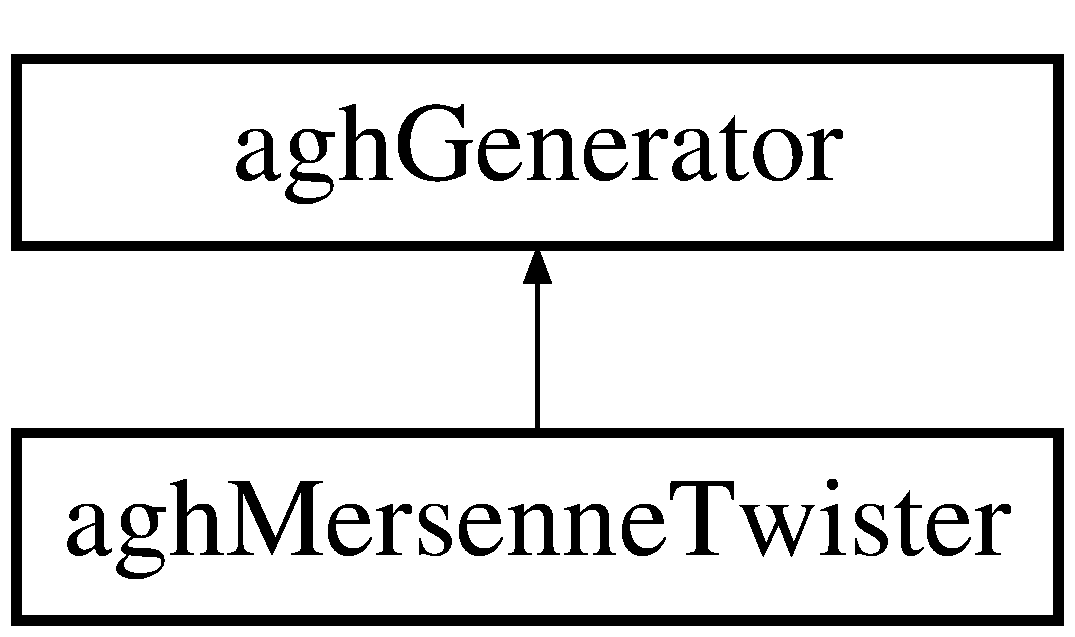
\includegraphics[height=2.000000cm]{classaghMersenneTwister}
\end{center}
\end{figure}
\subsection*{\-Public \-Member \-Functions}
\begin{DoxyCompactItemize}
\item 
\hypertarget{classaghMersenneTwister_a51589fc19681ec088c608cbf4b7a7ed5}{\hyperlink{classaghMersenneTwister_a51589fc19681ec088c608cbf4b7a7ed5}{agh\-Mersenne\-Twister} ()}\label{classaghMersenneTwister_a51589fc19681ec088c608cbf4b7a7ed5}

\begin{DoxyCompactList}\small\item\em \-Konstruktor bezparametrowy klasy. \end{DoxyCompactList}\item 
\hyperlink{classaghMersenneTwister_afc8d9cd5414df5fc737aaa118f3b8d47}{agh\-Mersenne\-Twister} (int \-\_\-poczatek\-Zakres, int \-\_\-koniec\-Zakres, int \-\_\-ziarno)
\begin{DoxyCompactList}\small\item\em \-Konstruktor parametrowy klasy. \end{DoxyCompactList}\item 
virtual void \hyperlink{classaghMersenneTwister_aadb2ebbce4d8efdb3de835b1e5e17189}{ustaw\-Ziarno} (int \-\_\-ziarno)
\begin{DoxyCompactList}\small\item\em \-Wirtualna funkcja ustawaijąca ziarno. \end{DoxyCompactList}\item 
virtual int \hyperlink{classaghMersenneTwister_a28d9c9f0008890376688bb49b81a2071}{losuj\-Liczbe} ()
\end{DoxyCompactItemize}


\subsection{\-Detailed \-Description}
\-Definicja klasy \hyperlink{classaghMersenneTwister}{agh\-Mersenne\-Twister}. 

\begin{DoxyAuthor}{\-Author}
\-Izabela Śmietana \& \-Krzysztof \-Spytkowski 
\end{DoxyAuthor}
\begin{DoxyDate}{\-Date}
16.\-05.\-2013 
\end{DoxyDate}


\subsection{\-Constructor \& \-Destructor \-Documentation}
\hypertarget{classaghMersenneTwister_afc8d9cd5414df5fc737aaa118f3b8d47}{\index{agh\-Mersenne\-Twister@{agh\-Mersenne\-Twister}!agh\-Mersenne\-Twister@{agh\-Mersenne\-Twister}}
\index{agh\-Mersenne\-Twister@{agh\-Mersenne\-Twister}!aghMersenneTwister@{agh\-Mersenne\-Twister}}
\subsubsection[{agh\-Mersenne\-Twister}]{\setlength{\rightskip}{0pt plus 5cm}{\bf agh\-Mersenne\-Twister\-::agh\-Mersenne\-Twister} (
\begin{DoxyParamCaption}
\item[{int}]{\-\_\-poczatek\-Zakres, }
\item[{int}]{\-\_\-koniec\-Zakres, }
\item[{int}]{\-\_\-ziarno}
\end{DoxyParamCaption}
)}}\label{classaghMersenneTwister_afc8d9cd5414df5fc737aaa118f3b8d47}


\-Konstruktor parametrowy klasy. 


\begin{DoxyParams}{\-Parameters}
{\em \-\_\-poczatek\-Zakres} & -\/ \-Poczatek zakresu losowanych liczb \\
\hline
{\em \-\_\-koniec\-Zakres} & -\/ \-Koniec zakresu losowanych liczb \\
\hline
{\em \-\_\-ziarno} & -\/ \-Ziarno \\
\hline
\end{DoxyParams}


\subsection{\-Member \-Function \-Documentation}
\hypertarget{classaghMersenneTwister_a28d9c9f0008890376688bb49b81a2071}{\index{agh\-Mersenne\-Twister@{agh\-Mersenne\-Twister}!losuj\-Liczbe@{losuj\-Liczbe}}
\index{losuj\-Liczbe@{losuj\-Liczbe}!aghMersenneTwister@{agh\-Mersenne\-Twister}}
\subsubsection[{losuj\-Liczbe}]{\setlength{\rightskip}{0pt plus 5cm}int {\bf agh\-Mersenne\-Twister\-::losuj\-Liczbe} (
\begin{DoxyParamCaption}
{}
\end{DoxyParamCaption}
)\hspace{0.3cm}{\ttfamily  \mbox{[}virtual\mbox{]}}}}\label{classaghMersenneTwister_a28d9c9f0008890376688bb49b81a2071}
\begin{DoxyReturn}{\-Returns}
\-Wylosowana liczba 
\end{DoxyReturn}


\-Implements \hyperlink{classaghGenerator_ae0f3bbfe8a7d233c006728c060a2e453}{agh\-Generator}.

\hypertarget{classaghMersenneTwister_aadb2ebbce4d8efdb3de835b1e5e17189}{\index{agh\-Mersenne\-Twister@{agh\-Mersenne\-Twister}!ustaw\-Ziarno@{ustaw\-Ziarno}}
\index{ustaw\-Ziarno@{ustaw\-Ziarno}!aghMersenneTwister@{agh\-Mersenne\-Twister}}
\subsubsection[{ustaw\-Ziarno}]{\setlength{\rightskip}{0pt plus 5cm}void {\bf agh\-Mersenne\-Twister\-::ustaw\-Ziarno} (
\begin{DoxyParamCaption}
\item[{int}]{\-\_\-ziarno}
\end{DoxyParamCaption}
)\hspace{0.3cm}{\ttfamily  \mbox{[}virtual\mbox{]}}}}\label{classaghMersenneTwister_aadb2ebbce4d8efdb3de835b1e5e17189}


\-Wirtualna funkcja ustawaijąca ziarno. 


\begin{DoxyParams}{\-Parameters}
{\em \-\_\-ziarno} & -\/ \-Ziarno \\
\hline
\end{DoxyParams}


\-Reimplemented from \hyperlink{classaghGenerator_aeb8309c8c8d14bb1df9a594776399a23}{agh\-Generator}.



\-The documentation for this class was generated from the following files\-:\begin{DoxyCompactItemize}
\item 
\hyperlink{aghMersenneTwister_8h}{agh\-Mersenne\-Twister.\-h}\item 
agh\-Mersenne\-Twister.\-cpp\end{DoxyCompactItemize}

\hypertarget{classaghPi}{\section{agh\-Pi \-Class \-Reference}
\label{classaghPi}\index{agh\-Pi@{agh\-Pi}}
}


\-Definicja klasy \hyperlink{classaghPi}{agh\-Pi}.  




{\ttfamily \#include $<$agh\-Pi.\-h$>$}

\-Inheritance diagram for agh\-Pi\-:\begin{figure}[H]
\begin{center}
\leavevmode
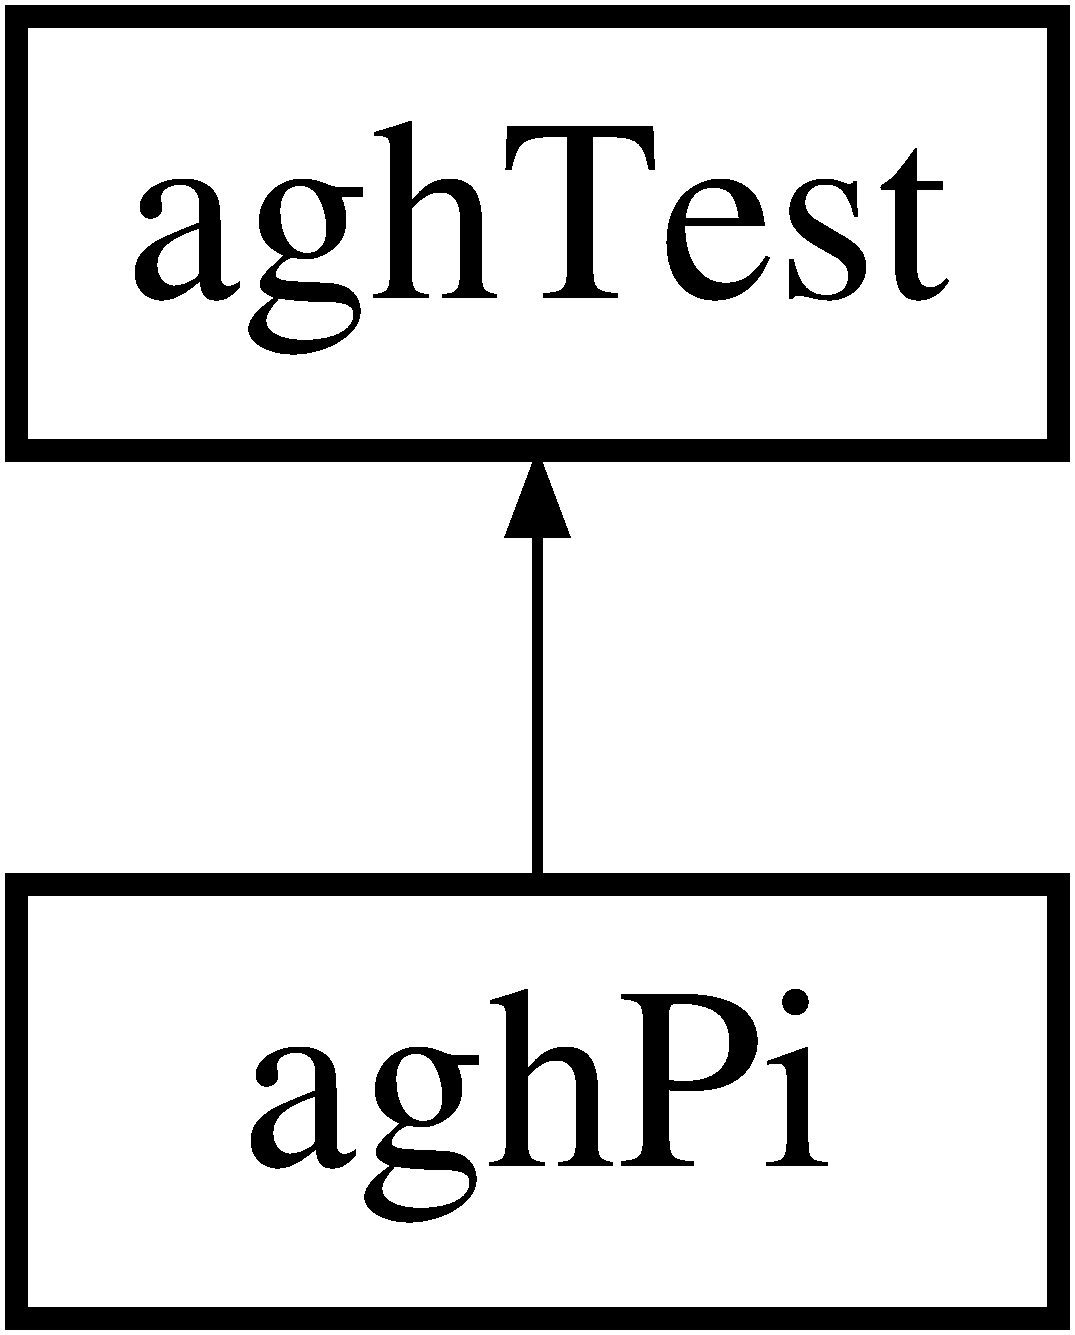
\includegraphics[height=2.000000cm]{classaghPi}
\end{center}
\end{figure}
\subsection*{\-Public \-Member \-Functions}
\begin{DoxyCompactItemize}
\item 
\hypertarget{classaghPi_aa71f972681e797f5c0ceaa03108a5405}{\hyperlink{classaghPi_aa71f972681e797f5c0ceaa03108a5405}{agh\-Pi} ()}\label{classaghPi_aa71f972681e797f5c0ceaa03108a5405}

\begin{DoxyCompactList}\small\item\em \-Konstruktor bezparametrowy klasy. \end{DoxyCompactList}\item 
\hyperlink{classaghPi_aa01f39d1292324113611a0d027b50844}{agh\-Pi} (\hyperlink{classaghGenerator}{agh\-Generator} $\ast$\-\_\-wsk\-Generator, int \-\_\-ilosc\-Liczb)
\begin{DoxyCompactList}\small\item\em \-Konstruktor parametrowy klasy. \end{DoxyCompactList}\item 
\hypertarget{classaghPi_a5c24506f0ba7143dc8423a747182f944}{virtual void \hyperlink{classaghPi_a5c24506f0ba7143dc8423a747182f944}{testuj} ()}\label{classaghPi_a5c24506f0ba7143dc8423a747182f944}

\begin{DoxyCompactList}\small\item\em \-Wirtualna funkcja testująca generator. \end{DoxyCompactList}\item 
virtual void \hyperlink{classaghPi_ab3647aaa2e951924447d755379d043b4}{wypisz} (ostream \&strumien=cout)
\begin{DoxyCompactList}\small\item\em \-Wirtualna funkcja wypisująca na zadany strumien wynik testu. \end{DoxyCompactList}\end{DoxyCompactItemize}
\subsection*{\-Static \-Public \-Attributes}
\begin{DoxyCompactItemize}
\item 
static const double \hyperlink{classaghPi_a28b57c723fa47234631aa425b3b1a40e}{pi} = 3.\-14159
\end{DoxyCompactItemize}


\subsection{\-Detailed \-Description}
\-Definicja klasy \hyperlink{classaghPi}{agh\-Pi}. 

\begin{DoxyAuthor}{\-Author}
\-Izabela Śmietana \& \-Krzysztof \-Spytkowski 
\end{DoxyAuthor}
\begin{DoxyDate}{\-Date}
16.\-05.\-2013 
\end{DoxyDate}


\subsection{\-Constructor \& \-Destructor \-Documentation}
\hypertarget{classaghPi_aa01f39d1292324113611a0d027b50844}{\index{agh\-Pi@{agh\-Pi}!agh\-Pi@{agh\-Pi}}
\index{agh\-Pi@{agh\-Pi}!aghPi@{agh\-Pi}}
\subsubsection[{agh\-Pi}]{\setlength{\rightskip}{0pt plus 5cm}{\bf agh\-Pi\-::agh\-Pi} (
\begin{DoxyParamCaption}
\item[{{\bf agh\-Generator} $\ast$}]{\-\_\-wsk\-Generator, }
\item[{int}]{\-\_\-ilosc\-Liczb}
\end{DoxyParamCaption}
)}}\label{classaghPi_aa01f39d1292324113611a0d027b50844}


\-Konstruktor parametrowy klasy. 


\begin{DoxyParams}{\-Parameters}
{\em \-\_\-wsk\-Generator} & -\/ \-Wskaźnik na generator \\
\hline
{\em \-\_\-ilosc\-Liczb} & -\/ \-Ilośc liczb do wylosowania \\
\hline
\end{DoxyParams}


\subsection{\-Member \-Function \-Documentation}
\hypertarget{classaghPi_ab3647aaa2e951924447d755379d043b4}{\index{agh\-Pi@{agh\-Pi}!wypisz@{wypisz}}
\index{wypisz@{wypisz}!aghPi@{agh\-Pi}}
\subsubsection[{wypisz}]{\setlength{\rightskip}{0pt plus 5cm}void {\bf agh\-Pi\-::wypisz} (
\begin{DoxyParamCaption}
\item[{ostream \&}]{strumien = {\ttfamily cout}}
\end{DoxyParamCaption}
)\hspace{0.3cm}{\ttfamily  \mbox{[}virtual\mbox{]}}}}\label{classaghPi_ab3647aaa2e951924447d755379d043b4}


\-Wirtualna funkcja wypisująca na zadany strumien wynik testu. 


\begin{DoxyParams}{\-Parameters}
{\em strumien} & -\/ \-Strumien, na który należy wypisać wynik testu (domyślnie cout) \\
\hline
\end{DoxyParams}


\-Implements \hyperlink{classaghTest_ad43c3c9a98d652936d9a5fe90aa1b57b}{agh\-Test}.



\subsection{\-Member \-Data \-Documentation}
\hypertarget{classaghPi_a28b57c723fa47234631aa425b3b1a40e}{\index{agh\-Pi@{agh\-Pi}!pi@{pi}}
\index{pi@{pi}!aghPi@{agh\-Pi}}
\subsubsection[{pi}]{\setlength{\rightskip}{0pt plus 5cm}const double {\bf agh\-Pi\-::pi} = 3.\-14159\hspace{0.3cm}{\ttfamily  \mbox{[}static\mbox{]}}}}\label{classaghPi_a28b57c723fa47234631aa425b3b1a40e}
\-Wzorcowa wartość liczby pi 

\-The documentation for this class was generated from the following files\-:\begin{DoxyCompactItemize}
\item 
\hyperlink{aghPi_8h}{agh\-Pi.\-h}\item 
agh\-Pi.\-cpp\end{DoxyCompactItemize}

\hypertarget{classaghSrednia}{\section{agh\-Srednia \-Class \-Reference}
\label{classaghSrednia}\index{agh\-Srednia@{agh\-Srednia}}
}


\-Definicja klasy \hyperlink{classaghSrednia}{agh\-Srednia}.  




{\ttfamily \#include $<$agh\-Srednia.\-h$>$}

\-Inheritance diagram for agh\-Srednia\-:\begin{figure}[H]
\begin{center}
\leavevmode
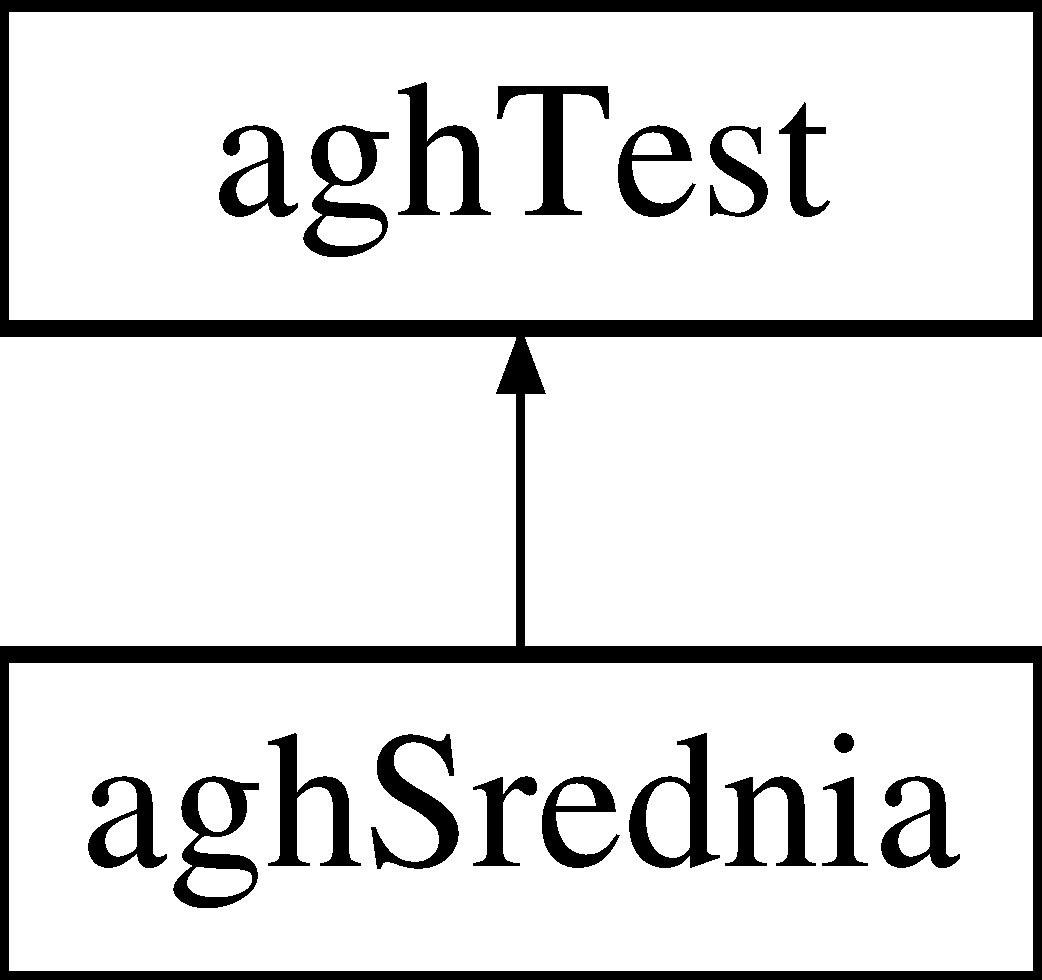
\includegraphics[height=2.000000cm]{classaghSrednia}
\end{center}
\end{figure}
\subsection*{\-Public \-Member \-Functions}
\begin{DoxyCompactItemize}
\item 
\hypertarget{classaghSrednia_a618c328f4f94e358bf8a6a09db4e992c}{\hyperlink{classaghSrednia_a618c328f4f94e358bf8a6a09db4e992c}{agh\-Srednia} ()}\label{classaghSrednia_a618c328f4f94e358bf8a6a09db4e992c}

\begin{DoxyCompactList}\small\item\em \-Konstruktor bezparametrowy klasy. \end{DoxyCompactList}\item 
\hyperlink{classaghSrednia_a8cadd31f7df514a19544561793b774b1}{agh\-Srednia} (\hyperlink{classaghGenerator}{agh\-Generator} $\ast$\-\_\-wsk\-Generator, int \-\_\-ilosc\-Liczb)
\begin{DoxyCompactList}\small\item\em \-Konstruktor parametrowy klasy. \end{DoxyCompactList}\item 
\hypertarget{classaghSrednia_a5b9c95e4cb2fcbd0c905bfe6839dedd4}{virtual void \hyperlink{classaghSrednia_a5b9c95e4cb2fcbd0c905bfe6839dedd4}{testuj} ()}\label{classaghSrednia_a5b9c95e4cb2fcbd0c905bfe6839dedd4}

\begin{DoxyCompactList}\small\item\em \-Wirtualna funkcja testująca generator. \end{DoxyCompactList}\item 
virtual void \hyperlink{classaghSrednia_ab66006aa06658abf55422d3629cf95f5}{wypisz} (ostream \&strumien=cout)
\begin{DoxyCompactList}\small\item\em \-Wirtualna funkcja wypisująca na zadany strumien wynik testu. \end{DoxyCompactList}\end{DoxyCompactItemize}


\subsection{\-Detailed \-Description}
\-Definicja klasy \hyperlink{classaghSrednia}{agh\-Srednia}. 

\begin{DoxyAuthor}{\-Author}
\-Izabela Śmietana \& \-Krzysztof \-Spytkowski 
\end{DoxyAuthor}
\begin{DoxyDate}{\-Date}
16.\-05.\-2013 
\end{DoxyDate}


\subsection{\-Constructor \& \-Destructor \-Documentation}
\hypertarget{classaghSrednia_a8cadd31f7df514a19544561793b774b1}{\index{agh\-Srednia@{agh\-Srednia}!agh\-Srednia@{agh\-Srednia}}
\index{agh\-Srednia@{agh\-Srednia}!aghSrednia@{agh\-Srednia}}
\subsubsection[{agh\-Srednia}]{\setlength{\rightskip}{0pt plus 5cm}{\bf agh\-Srednia\-::agh\-Srednia} (
\begin{DoxyParamCaption}
\item[{{\bf agh\-Generator} $\ast$}]{\-\_\-wsk\-Generator, }
\item[{int}]{\-\_\-ilosc\-Liczb}
\end{DoxyParamCaption}
)}}\label{classaghSrednia_a8cadd31f7df514a19544561793b774b1}


\-Konstruktor parametrowy klasy. 


\begin{DoxyParams}{\-Parameters}
{\em \-\_\-wsk\-Generator} & -\/ \-Wskaźnik na generator \\
\hline
{\em \-\_\-ilosc\-Liczb} & -\/ \-Ilośc liczb do wylosowania \\
\hline
\end{DoxyParams}


\subsection{\-Member \-Function \-Documentation}
\hypertarget{classaghSrednia_ab66006aa06658abf55422d3629cf95f5}{\index{agh\-Srednia@{agh\-Srednia}!wypisz@{wypisz}}
\index{wypisz@{wypisz}!aghSrednia@{agh\-Srednia}}
\subsubsection[{wypisz}]{\setlength{\rightskip}{0pt plus 5cm}void {\bf agh\-Srednia\-::wypisz} (
\begin{DoxyParamCaption}
\item[{ostream \&}]{strumien = {\ttfamily cout}}
\end{DoxyParamCaption}
)\hspace{0.3cm}{\ttfamily  \mbox{[}virtual\mbox{]}}}}\label{classaghSrednia_ab66006aa06658abf55422d3629cf95f5}


\-Wirtualna funkcja wypisująca na zadany strumien wynik testu. 


\begin{DoxyParams}{\-Parameters}
{\em strumien} & -\/ \-Strumien, na który należy wypisać wynik testu (domyślnie cout) \\
\hline
\end{DoxyParams}


\-Implements \hyperlink{classaghTest_ad43c3c9a98d652936d9a5fe90aa1b57b}{agh\-Test}.



\-The documentation for this class was generated from the following files\-:\begin{DoxyCompactItemize}
\item 
\hyperlink{aghSrednia_8h}{agh\-Srednia.\-h}\item 
agh\-Srednia.\-cpp\end{DoxyCompactItemize}

\hypertarget{classaghTest}{\section{agh\-Test \-Class \-Reference}
\label{classaghTest}\index{agh\-Test@{agh\-Test}}
}


\-Definicja klasy abstrakcyjnej \hyperlink{classaghTest}{agh\-Test}.  




{\ttfamily \#include $<$agh\-Test.\-h$>$}

\-Inheritance diagram for agh\-Test\-:\begin{figure}[H]
\begin{center}
\leavevmode
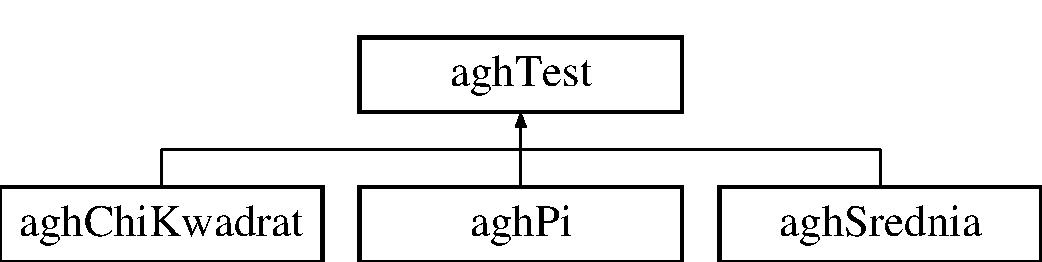
\includegraphics[height=2.000000cm]{classaghTest}
\end{center}
\end{figure}
\subsection*{\-Public \-Member \-Functions}
\begin{DoxyCompactItemize}
\item 
\hypertarget{classaghTest_ad401b4396042eec67f799a3321c24da6}{\hyperlink{classaghTest_ad401b4396042eec67f799a3321c24da6}{agh\-Test} ()}\label{classaghTest_ad401b4396042eec67f799a3321c24da6}

\begin{DoxyCompactList}\small\item\em \-Konstruktor bezparametrowy klasy. \end{DoxyCompactList}\item 
\hyperlink{classaghTest_a1e64dbd5d26b0852983b94fee03d3acf}{agh\-Test} (\hyperlink{classaghGenerator}{agh\-Generator} $\ast$\-\_\-wsk\-Generator, int \-\_\-ilosc\-Liczb)
\begin{DoxyCompactList}\small\item\em \-Konstruktor parametrowy klasy. \end{DoxyCompactList}\item 
\hypertarget{classaghTest_ae4906739e0f9e889febd23a43803b481}{virtual \hyperlink{classaghTest_ae4906739e0f9e889febd23a43803b481}{$\sim$agh\-Test} ()}\label{classaghTest_ae4906739e0f9e889febd23a43803b481}

\begin{DoxyCompactList}\small\item\em \-Wirtualny destruktor klasy. \end{DoxyCompactList}\item 
void \hyperlink{classaghTest_a971401190c3ddb295c8f09fe40291ae7}{ustaw\-Generator} (\hyperlink{classaghGenerator}{agh\-Generator} $\ast$\-\_\-wsk\-Generator)
\begin{DoxyCompactList}\small\item\em \-Funkcja ustawaijąca wskaźnik na generator. \end{DoxyCompactList}\item 
void \hyperlink{classaghTest_a69b1abb67e748e5077c0d8dbf798bb95}{ustaw\-Ilosc\-Liczb} (int \-\_\-ilosc\-Liczb)
\begin{DoxyCompactList}\small\item\em \-Funkcja ustawaijąca ilośc liczb do wylosowania. \end{DoxyCompactList}\item 
\hypertarget{classaghTest_aedc07452db24c0b2389599fbb5a25e03}{virtual void \hyperlink{classaghTest_aedc07452db24c0b2389599fbb5a25e03}{testuj} ()=0}\label{classaghTest_aedc07452db24c0b2389599fbb5a25e03}

\begin{DoxyCompactList}\small\item\em \-Czysto wirtualna funkcja testująca generator. \end{DoxyCompactList}\item 
void \hyperlink{classaghTest_aa278aea7075db6ddf520b193038265a5}{wypisz\-Nazwe} (ostream \&strumien=cout)
\begin{DoxyCompactList}\small\item\em \-Funkcja wypisująca na zadany strumien nazwe testu. \end{DoxyCompactList}\item 
virtual void \hyperlink{classaghTest_ad43c3c9a98d652936d9a5fe90aa1b57b}{wypisz} (ostream \&strumien=cout)=0
\begin{DoxyCompactList}\small\item\em \-Czysto wirtualna funkcja wypisująca na zadany strumien wynik testu. \end{DoxyCompactList}\end{DoxyCompactItemize}
\subsection*{\-Protected \-Attributes}
\begin{DoxyCompactItemize}
\item 
\hypertarget{classaghTest_a857cc9a7264a6c91d570dca932b170a1}{\hyperlink{classaghGenerator}{agh\-Generator} $\ast$ \hyperlink{classaghTest_a857cc9a7264a6c91d570dca932b170a1}{wsk\-Generator}}\label{classaghTest_a857cc9a7264a6c91d570dca932b170a1}

\begin{DoxyCompactList}\small\item\em \-Wskaźnik na generator. \end{DoxyCompactList}\item 
\hypertarget{classaghTest_ac7b2b561a6c98219dd5ba7a7e24bd1d9}{int \hyperlink{classaghTest_ac7b2b561a6c98219dd5ba7a7e24bd1d9}{ilosc\-Liczb}}\label{classaghTest_ac7b2b561a6c98219dd5ba7a7e24bd1d9}

\begin{DoxyCompactList}\small\item\em \-Ilośc liczb do wylosowania. \end{DoxyCompactList}\item 
\hypertarget{classaghTest_a81d6064593d5da46e32f4e1ecdc45550}{const char $\ast$ \hyperlink{classaghTest_a81d6064593d5da46e32f4e1ecdc45550}{nazwa\-Test}}\label{classaghTest_a81d6064593d5da46e32f4e1ecdc45550}

\begin{DoxyCompactList}\small\item\em \-Nazwa testu. \end{DoxyCompactList}\end{DoxyCompactItemize}


\subsection{\-Detailed \-Description}
\-Definicja klasy abstrakcyjnej \hyperlink{classaghTest}{agh\-Test}. 

\begin{DoxyAuthor}{\-Author}
\-Izabela Śmietana \& \-Krzysztof \-Spytkowski 
\end{DoxyAuthor}
\begin{DoxyDate}{\-Date}
16.\-05.\-2013 
\end{DoxyDate}


\subsection{\-Constructor \& \-Destructor \-Documentation}
\hypertarget{classaghTest_a1e64dbd5d26b0852983b94fee03d3acf}{\index{agh\-Test@{agh\-Test}!agh\-Test@{agh\-Test}}
\index{agh\-Test@{agh\-Test}!aghTest@{agh\-Test}}
\subsubsection[{agh\-Test}]{\setlength{\rightskip}{0pt plus 5cm}{\bf agh\-Test\-::agh\-Test} (
\begin{DoxyParamCaption}
\item[{{\bf agh\-Generator} $\ast$}]{\-\_\-wsk\-Generator, }
\item[{int}]{\-\_\-ilosc\-Liczb}
\end{DoxyParamCaption}
)}}\label{classaghTest_a1e64dbd5d26b0852983b94fee03d3acf}


\-Konstruktor parametrowy klasy. 


\begin{DoxyParams}{\-Parameters}
{\em \-\_\-wsk\-Generator} & -\/ \-Wskaźnik na generator \\
\hline
{\em \-\_\-ilosc\-Liczb} & -\/ \-Ilośc liczb do wylosowania \\
\hline
\end{DoxyParams}


\subsection{\-Member \-Function \-Documentation}
\hypertarget{classaghTest_a971401190c3ddb295c8f09fe40291ae7}{\index{agh\-Test@{agh\-Test}!ustaw\-Generator@{ustaw\-Generator}}
\index{ustaw\-Generator@{ustaw\-Generator}!aghTest@{agh\-Test}}
\subsubsection[{ustaw\-Generator}]{\setlength{\rightskip}{0pt plus 5cm}void {\bf agh\-Test\-::ustaw\-Generator} (
\begin{DoxyParamCaption}
\item[{{\bf agh\-Generator} $\ast$}]{\-\_\-wsk\-Generator}
\end{DoxyParamCaption}
)}}\label{classaghTest_a971401190c3ddb295c8f09fe40291ae7}


\-Funkcja ustawaijąca wskaźnik na generator. 


\begin{DoxyParams}{\-Parameters}
{\em \-\_\-wsk\-Generator} & -\/ \-Wskaźnik na generator \\
\hline
\end{DoxyParams}
\hypertarget{classaghTest_a69b1abb67e748e5077c0d8dbf798bb95}{\index{agh\-Test@{agh\-Test}!ustaw\-Ilosc\-Liczb@{ustaw\-Ilosc\-Liczb}}
\index{ustaw\-Ilosc\-Liczb@{ustaw\-Ilosc\-Liczb}!aghTest@{agh\-Test}}
\subsubsection[{ustaw\-Ilosc\-Liczb}]{\setlength{\rightskip}{0pt plus 5cm}void {\bf agh\-Test\-::ustaw\-Ilosc\-Liczb} (
\begin{DoxyParamCaption}
\item[{int}]{\-\_\-ilosc\-Liczb}
\end{DoxyParamCaption}
)}}\label{classaghTest_a69b1abb67e748e5077c0d8dbf798bb95}


\-Funkcja ustawaijąca ilośc liczb do wylosowania. 


\begin{DoxyParams}{\-Parameters}
{\em \-\_\-ilosc\-Liczb} & -\/ \-Ilośc liczb do wylosowania \\
\hline
\end{DoxyParams}
\hypertarget{classaghTest_ad43c3c9a98d652936d9a5fe90aa1b57b}{\index{agh\-Test@{agh\-Test}!wypisz@{wypisz}}
\index{wypisz@{wypisz}!aghTest@{agh\-Test}}
\subsubsection[{wypisz}]{\setlength{\rightskip}{0pt plus 5cm}virtual void {\bf agh\-Test\-::wypisz} (
\begin{DoxyParamCaption}
\item[{ostream \&}]{strumien = {\ttfamily cout}}
\end{DoxyParamCaption}
)\hspace{0.3cm}{\ttfamily  \mbox{[}pure virtual\mbox{]}}}}\label{classaghTest_ad43c3c9a98d652936d9a5fe90aa1b57b}


\-Czysto wirtualna funkcja wypisująca na zadany strumien wynik testu. 


\begin{DoxyParams}{\-Parameters}
{\em strumien} & -\/ \-Strumien, na który należy wypisać wynik testu (domyślnie cout) \\
\hline
\end{DoxyParams}


\-Implemented in \hyperlink{classaghChiKwadrat_a6d86b271437ada0f232164812a3671c5}{agh\-Chi\-Kwadrat}, \hyperlink{classaghPi_ab3647aaa2e951924447d755379d043b4}{agh\-Pi}, and \hyperlink{classaghSrednia_ab66006aa06658abf55422d3629cf95f5}{agh\-Srednia}.

\hypertarget{classaghTest_aa278aea7075db6ddf520b193038265a5}{\index{agh\-Test@{agh\-Test}!wypisz\-Nazwe@{wypisz\-Nazwe}}
\index{wypisz\-Nazwe@{wypisz\-Nazwe}!aghTest@{agh\-Test}}
\subsubsection[{wypisz\-Nazwe}]{\setlength{\rightskip}{0pt plus 5cm}void {\bf agh\-Test\-::wypisz\-Nazwe} (
\begin{DoxyParamCaption}
\item[{ostream \&}]{strumien = {\ttfamily cout}}
\end{DoxyParamCaption}
)}}\label{classaghTest_aa278aea7075db6ddf520b193038265a5}


\-Funkcja wypisująca na zadany strumien nazwe testu. 


\begin{DoxyParams}{\-Parameters}
{\em strumien} & -\/ \-Strumien, na który należy wypisać nazwe testu (domyślnie cout) \\
\hline
\end{DoxyParams}


\-The documentation for this class was generated from the following files\-:\begin{DoxyCompactItemize}
\item 
\hyperlink{aghTest_8h}{agh\-Test.\-h}\item 
agh\-Test.\-cpp\end{DoxyCompactItemize}

\hypertarget{classaghWbudowany}{\section{agh\-Wbudowany \-Class \-Reference}
\label{classaghWbudowany}\index{agh\-Wbudowany@{agh\-Wbudowany}}
}


\-Definicja klasy \hyperlink{classaghWbudowany}{agh\-Wbudowany}.  




{\ttfamily \#include $<$agh\-Wbudowany.\-h$>$}

\-Inheritance diagram for agh\-Wbudowany\-:\begin{figure}[H]
\begin{center}
\leavevmode
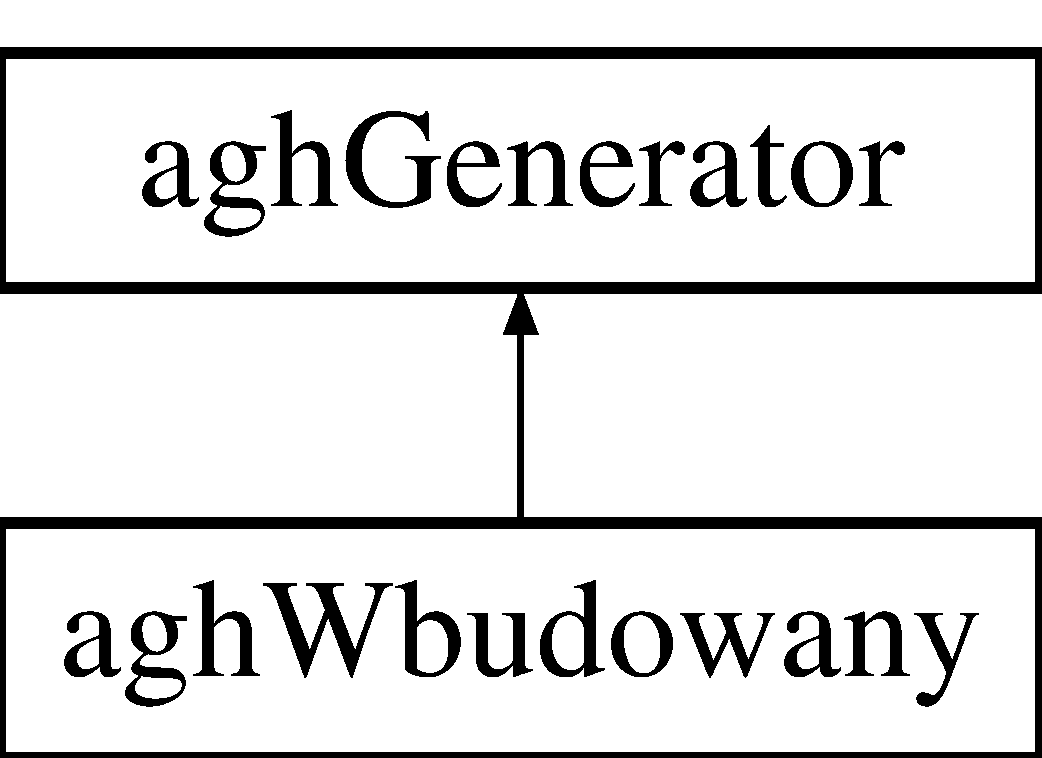
\includegraphics[height=2.000000cm]{classaghWbudowany}
\end{center}
\end{figure}
\subsection*{\-Public \-Member \-Functions}
\begin{DoxyCompactItemize}
\item 
\hypertarget{classaghWbudowany_a74ef28fbbe2b8563c6fd2f2c7acbdbe5}{\hyperlink{classaghWbudowany_a74ef28fbbe2b8563c6fd2f2c7acbdbe5}{agh\-Wbudowany} ()}\label{classaghWbudowany_a74ef28fbbe2b8563c6fd2f2c7acbdbe5}

\begin{DoxyCompactList}\small\item\em \-Konstruktor bezparametrowy klasy. \end{DoxyCompactList}\item 
\hyperlink{classaghWbudowany_a50e3179651d25e86e277a2d18a5c6859}{agh\-Wbudowany} (int \-\_\-poczatek\-Zakres, int \-\_\-koniec\-Zakres, int \-\_\-ziarno)
\begin{DoxyCompactList}\small\item\em \-Konstruktor parametrowy klasy. \end{DoxyCompactList}\item 
virtual void \hyperlink{classaghWbudowany_a5d636a572dde32c97ba398420aa1afac}{ustaw\-Ziarno} (int \-\_\-ziarno)
\begin{DoxyCompactList}\small\item\em \-Wirtualna funkcja ustawaijąca ziarno. \end{DoxyCompactList}\item 
virtual int \hyperlink{classaghWbudowany_adcf9ea98875775913421076e4c277e56}{losuj\-Liczbe} ()
\end{DoxyCompactItemize}


\subsection{\-Detailed \-Description}
\-Definicja klasy \hyperlink{classaghWbudowany}{agh\-Wbudowany}. 

\begin{DoxyAuthor}{\-Author}
\-Izabela Śmietana \& \-Krzysztof \-Spytkowski 
\end{DoxyAuthor}
\begin{DoxyDate}{\-Date}
16.\-05.\-2013 
\end{DoxyDate}


\subsection{\-Constructor \& \-Destructor \-Documentation}
\hypertarget{classaghWbudowany_a50e3179651d25e86e277a2d18a5c6859}{\index{agh\-Wbudowany@{agh\-Wbudowany}!agh\-Wbudowany@{agh\-Wbudowany}}
\index{agh\-Wbudowany@{agh\-Wbudowany}!aghWbudowany@{agh\-Wbudowany}}
\subsubsection[{agh\-Wbudowany}]{\setlength{\rightskip}{0pt plus 5cm}{\bf agh\-Wbudowany\-::agh\-Wbudowany} (
\begin{DoxyParamCaption}
\item[{int}]{\-\_\-poczatek\-Zakres, }
\item[{int}]{\-\_\-koniec\-Zakres, }
\item[{int}]{\-\_\-ziarno}
\end{DoxyParamCaption}
)}}\label{classaghWbudowany_a50e3179651d25e86e277a2d18a5c6859}


\-Konstruktor parametrowy klasy. 


\begin{DoxyParams}{\-Parameters}
{\em \-\_\-poczatek\-Zakres} & -\/ \-Poczatek zakresu losowanych liczb \\
\hline
{\em \-\_\-koniec\-Zakres} & -\/ \-Koniec zakresu losowanych liczb \\
\hline
{\em \-\_\-ziarno} & -\/ \-Ziarno \\
\hline
\end{DoxyParams}


\subsection{\-Member \-Function \-Documentation}
\hypertarget{classaghWbudowany_adcf9ea98875775913421076e4c277e56}{\index{agh\-Wbudowany@{agh\-Wbudowany}!losuj\-Liczbe@{losuj\-Liczbe}}
\index{losuj\-Liczbe@{losuj\-Liczbe}!aghWbudowany@{agh\-Wbudowany}}
\subsubsection[{losuj\-Liczbe}]{\setlength{\rightskip}{0pt plus 5cm}int {\bf agh\-Wbudowany\-::losuj\-Liczbe} (
\begin{DoxyParamCaption}
{}
\end{DoxyParamCaption}
)\hspace{0.3cm}{\ttfamily  \mbox{[}virtual\mbox{]}}}}\label{classaghWbudowany_adcf9ea98875775913421076e4c277e56}
\begin{DoxyReturn}{\-Returns}
\-Wylosowana liczba 
\end{DoxyReturn}


\-Implements \hyperlink{classaghGenerator_ae0f3bbfe8a7d233c006728c060a2e453}{agh\-Generator}.

\hypertarget{classaghWbudowany_a5d636a572dde32c97ba398420aa1afac}{\index{agh\-Wbudowany@{agh\-Wbudowany}!ustaw\-Ziarno@{ustaw\-Ziarno}}
\index{ustaw\-Ziarno@{ustaw\-Ziarno}!aghWbudowany@{agh\-Wbudowany}}
\subsubsection[{ustaw\-Ziarno}]{\setlength{\rightskip}{0pt plus 5cm}void {\bf agh\-Wbudowany\-::ustaw\-Ziarno} (
\begin{DoxyParamCaption}
\item[{int}]{\-\_\-ziarno}
\end{DoxyParamCaption}
)\hspace{0.3cm}{\ttfamily  \mbox{[}virtual\mbox{]}}}}\label{classaghWbudowany_a5d636a572dde32c97ba398420aa1afac}


\-Wirtualna funkcja ustawaijąca ziarno. 


\begin{DoxyParams}{\-Parameters}
{\em \-\_\-ziarno} & -\/ \-Ziarno \\
\hline
\end{DoxyParams}


\-Reimplemented from \hyperlink{classaghGenerator_aeb8309c8c8d14bb1df9a594776399a23}{agh\-Generator}.



\-The documentation for this class was generated from the following files\-:\begin{DoxyCompactItemize}
\item 
\hyperlink{aghWbudowany_8h}{agh\-Wbudowany.\-h}\item 
agh\-Wbudowany.\-cpp\end{DoxyCompactItemize}

\chapter{\-File \-Documentation}
\hypertarget{aghBlumBlumShub_8h}{\section{agh\-Blum\-Blum\-Shub.\-h \-File \-Reference}
\label{aghBlumBlumShub_8h}\index{agh\-Blum\-Blum\-Shub.\-h@{agh\-Blum\-Blum\-Shub.\-h}}
}


\-Plik zawiera deklaracje klasy \hyperlink{classaghBlumBlumShub}{agh\-Blum\-Blum\-Shub}.  


{\ttfamily \#include \char`\"{}agh\-Generator.\-h\char`\"{}}\*
{\ttfamily \#include $<$cmath$>$}\*
\subsection*{\-Classes}
\begin{DoxyCompactItemize}
\item 
class \hyperlink{classaghBlumBlumShub}{agh\-Blum\-Blum\-Shub}
\begin{DoxyCompactList}\small\item\em \-Definicja klasy \hyperlink{classaghBlumBlumShub}{agh\-Blum\-Blum\-Shub}. \end{DoxyCompactList}\end{DoxyCompactItemize}


\subsection{\-Detailed \-Description}
\-Plik zawiera deklaracje klasy \hyperlink{classaghBlumBlumShub}{agh\-Blum\-Blum\-Shub}. \begin{DoxyAuthor}{\-Author}
\-Izabela Śmietana \& \-Krzysztof \-Spytkowski 
\end{DoxyAuthor}
\begin{DoxyDate}{\-Date}
16.\-05.\-2013 
\end{DoxyDate}
\begin{DoxyVersion}{\-Version}
1.\-0 
\end{DoxyVersion}

\hypertarget{aghChiKwadrat_8h}{\section{agh\-Chi\-Kwadrat.\-h \-File \-Reference}
\label{aghChiKwadrat_8h}\index{agh\-Chi\-Kwadrat.\-h@{agh\-Chi\-Kwadrat.\-h}}
}


\-Plik zawiera deklaracje klasy \hyperlink{classaghChiKwadrat}{agh\-Chi\-Kwadrat}.  


{\ttfamily \#include $<$cmath$>$}\*
{\ttfamily \#include \char`\"{}agh\-Test.\-h\char`\"{}}\*
\subsection*{\-Classes}
\begin{DoxyCompactItemize}
\item 
class \hyperlink{classaghChiKwadrat}{agh\-Chi\-Kwadrat}
\begin{DoxyCompactList}\small\item\em \-Definicja klasy \hyperlink{classaghChiKwadrat}{agh\-Chi\-Kwadrat}. \end{DoxyCompactList}\end{DoxyCompactItemize}


\subsection{\-Detailed \-Description}
\-Plik zawiera deklaracje klasy \hyperlink{classaghChiKwadrat}{agh\-Chi\-Kwadrat}. \begin{DoxyAuthor}{\-Author}
\-Izabela Śmietana \& \-Krzysztof \-Spytkowski 
\end{DoxyAuthor}
\begin{DoxyDate}{\-Date}
16.\-05.\-2013 
\end{DoxyDate}
\begin{DoxyVersion}{\-Version}
1.\-0 
\end{DoxyVersion}

\hypertarget{aghException_8h}{\section{agh\-Exception.\-h \-File \-Reference}
\label{aghException_8h}\index{agh\-Exception.\-h@{agh\-Exception.\-h}}
}


\-The definition of \hyperlink{classaghException}{agh\-Exception} class that allows for exception handling.  


{\ttfamily \#include $<$iostream$>$}\*
{\ttfamily \#include $<$string.\-h$>$}\*
\subsection*{\-Classes}
\begin{DoxyCompactItemize}
\item 
class \hyperlink{classaghException}{agh\-Exception}
\begin{DoxyCompactList}\small\item\em \-The definition of \hyperlink{classaghException}{agh\-Exception} class that allows for exception handling. \end{DoxyCompactList}\end{DoxyCompactItemize}
\subsection*{\-Functions}
\begin{DoxyCompactItemize}
\item 
ostream \& \hyperlink{aghException_8h_a10c70066bf9a72136e183f7fe9ecc9ea}{operator$<$$<$} (ostream \&\-\_\-\-\_\-out, \hyperlink{classaghException}{agh\-Exception} \&\-\_\-\-\_\-exception)
\begin{DoxyCompactList}\small\item\em an overloaded operator $<$$<$ that writes the error parameters to the given stream \end{DoxyCompactList}\end{DoxyCompactItemize}


\subsection{\-Detailed \-Description}
\-The definition of \hyperlink{classaghException}{agh\-Exception} class that allows for exception handling. \begin{DoxyAuthor}{\-Author}
\-Krzysztof \-Kaczor 
\end{DoxyAuthor}
\begin{DoxyDate}{\-Date}
15.\-04.\-2011 
\end{DoxyDate}
\begin{DoxyVersion}{\-Version}
1.\-0 
\end{DoxyVersion}


\subsection{\-Function \-Documentation}
\hypertarget{aghException_8h_a10c70066bf9a72136e183f7fe9ecc9ea}{\index{agh\-Exception.\-h@{agh\-Exception.\-h}!operator$<$$<$@{operator$<$$<$}}
\index{operator$<$$<$@{operator$<$$<$}!aghException.h@{agh\-Exception.\-h}}
\subsubsection[{operator$<$$<$}]{\setlength{\rightskip}{0pt plus 5cm}ostream\& operator$<$$<$ (
\begin{DoxyParamCaption}
\item[{ostream \&}]{\-\_\-\-\_\-out, }
\item[{{\bf agh\-Exception} \&}]{\-\_\-\-\_\-exception}
\end{DoxyParamCaption}
)}}\label{aghException_8h_a10c70066bf9a72136e183f7fe9ecc9ea}


an overloaded operator $<$$<$ that writes the error parameters to the given stream 


\begin{DoxyParams}{\-Parameters}
{\em \-\_\-\-\_\-out} & -\/ a given stream (display, file, etc.) \\
\hline
{\em \-\_\-\-\_\-exception} & -\/ a reference to the exception object \\
\hline
\end{DoxyParams}
\begin{DoxyReturn}{\-Returns}
returns a reference to the given stream 
\end{DoxyReturn}

\hypertarget{aghGenerator_8h}{\section{agh\-Generator.\-h \-File \-Reference}
\label{aghGenerator_8h}\index{agh\-Generator.\-h@{agh\-Generator.\-h}}
}


\-Plik zawiera deklaracje klasy abstrakcyjnej \hyperlink{classaghGenerator}{agh\-Generator}.  


{\ttfamily \#include $<$iostream$>$}\*
{\ttfamily \#include \char`\"{}agh\-Exception.\-h\char`\"{}}\*
\subsection*{\-Classes}
\begin{DoxyCompactItemize}
\item 
class \hyperlink{classaghGenerator}{agh\-Generator}
\begin{DoxyCompactList}\small\item\em \-Definicja klasy abstrakcyjnej \hyperlink{classaghGenerator}{agh\-Generator}. \end{DoxyCompactList}\end{DoxyCompactItemize}


\subsection{\-Detailed \-Description}
\-Plik zawiera deklaracje klasy abstrakcyjnej \hyperlink{classaghGenerator}{agh\-Generator}. \begin{DoxyAuthor}{\-Author}
\-Izabela Śmietana \& \-Krzysztof \-Spytkowski 
\end{DoxyAuthor}
\begin{DoxyDate}{\-Date}
16.\-05.\-2013 
\end{DoxyDate}
\begin{DoxyVersion}{\-Version}
1.\-0 
\end{DoxyVersion}

\hypertarget{aghMersenneTwister_8h}{\section{agh\-Mersenne\-Twister.\-h \-File \-Reference}
\label{aghMersenneTwister_8h}\index{agh\-Mersenne\-Twister.\-h@{agh\-Mersenne\-Twister.\-h}}
}


\-Plik zawiera deklaracje klasy \hyperlink{classaghMersenneTwister}{agh\-Mersenne\-Twister}.  


{\ttfamily \#include \char`\"{}agh\-Generator.\-h\char`\"{}}\*
\subsection*{\-Classes}
\begin{DoxyCompactItemize}
\item 
class \hyperlink{classaghMersenneTwister}{agh\-Mersenne\-Twister}
\begin{DoxyCompactList}\small\item\em \-Definicja klasy \hyperlink{classaghMersenneTwister}{agh\-Mersenne\-Twister}. \end{DoxyCompactList}\end{DoxyCompactItemize}


\subsection{\-Detailed \-Description}
\-Plik zawiera deklaracje klasy \hyperlink{classaghMersenneTwister}{agh\-Mersenne\-Twister}. \begin{DoxyAuthor}{\-Author}
\-Izabela Śmietana \& \-Krzysztof \-Spytkowski 
\end{DoxyAuthor}
\begin{DoxyDate}{\-Date}
16.\-05.\-2013 
\end{DoxyDate}
\begin{DoxyVersion}{\-Version}
1.\-0 
\end{DoxyVersion}

\hypertarget{aghPi_8h}{\section{agh\-Pi.\-h \-File \-Reference}
\label{aghPi_8h}\index{agh\-Pi.\-h@{agh\-Pi.\-h}}
}


\-Plik zawiera deklaracje klasy \hyperlink{classaghPi}{agh\-Pi}.  


{\ttfamily \#include \char`\"{}agh\-Test.\-h\char`\"{}}\*
\subsection*{\-Classes}
\begin{DoxyCompactItemize}
\item 
class \hyperlink{classaghPi}{agh\-Pi}
\begin{DoxyCompactList}\small\item\em \-Definicja klasy \hyperlink{classaghPi}{agh\-Pi}. \end{DoxyCompactList}\end{DoxyCompactItemize}


\subsection{\-Detailed \-Description}
\-Plik zawiera deklaracje klasy \hyperlink{classaghPi}{agh\-Pi}. \begin{DoxyAuthor}{\-Author}
\-Izabela Śmietana \& \-Krzysztof \-Spytkowski 
\end{DoxyAuthor}
\begin{DoxyDate}{\-Date}
16.\-05.\-2013 
\end{DoxyDate}
\begin{DoxyVersion}{\-Version}
1.\-0 
\end{DoxyVersion}

\hypertarget{aghSrednia_8h}{\section{agh\-Srednia.\-h \-File \-Reference}
\label{aghSrednia_8h}\index{agh\-Srednia.\-h@{agh\-Srednia.\-h}}
}


\-Plik zawiera deklaracje klasy \hyperlink{classaghSrednia}{agh\-Srednia}.  


{\ttfamily \#include \char`\"{}agh\-Test.\-h\char`\"{}}\*
\subsection*{\-Classes}
\begin{DoxyCompactItemize}
\item 
class \hyperlink{classaghSrednia}{agh\-Srednia}
\begin{DoxyCompactList}\small\item\em \-Definicja klasy \hyperlink{classaghSrednia}{agh\-Srednia}. \end{DoxyCompactList}\end{DoxyCompactItemize}


\subsection{\-Detailed \-Description}
\-Plik zawiera deklaracje klasy \hyperlink{classaghSrednia}{agh\-Srednia}. \begin{DoxyAuthor}{\-Author}
\-Izabela Śmietana \& \-Krzysztof \-Spytkowski 
\end{DoxyAuthor}
\begin{DoxyDate}{\-Date}
16.\-05.\-2013 
\end{DoxyDate}
\begin{DoxyVersion}{\-Version}
1.\-0 
\end{DoxyVersion}

\hypertarget{aghTest_8h}{\section{agh\-Test.\-h \-File \-Reference}
\label{aghTest_8h}\index{agh\-Test.\-h@{agh\-Test.\-h}}
}


\-Plik zawiera deklaracje klasy abstrakcyjnej \hyperlink{classaghTest}{agh\-Test}.  


{\ttfamily \#include $<$iostream$>$}\*
{\ttfamily \#include \char`\"{}agh\-Generator.\-h\char`\"{}}\*
\subsection*{\-Classes}
\begin{DoxyCompactItemize}
\item 
class \hyperlink{classaghTest}{agh\-Test}
\begin{DoxyCompactList}\small\item\em \-Definicja klasy abstrakcyjnej \hyperlink{classaghTest}{agh\-Test}. \end{DoxyCompactList}\end{DoxyCompactItemize}


\subsection{\-Detailed \-Description}
\-Plik zawiera deklaracje klasy abstrakcyjnej \hyperlink{classaghTest}{agh\-Test}. \begin{DoxyAuthor}{\-Author}
\-Izabela Śmietana \& \-Krzysztof \-Spytkowski 
\end{DoxyAuthor}
\begin{DoxyDate}{\-Date}
16.\-05.\-2013 
\end{DoxyDate}
\begin{DoxyVersion}{\-Version}
1.\-0 
\end{DoxyVersion}

\hypertarget{aghWbudowany_8h}{\section{agh\-Wbudowany.\-h \-File \-Reference}
\label{aghWbudowany_8h}\index{agh\-Wbudowany.\-h@{agh\-Wbudowany.\-h}}
}


\-Plik zawiera deklaracje klasy \hyperlink{classaghWbudowany}{agh\-Wbudowany}.  


{\ttfamily \#include \char`\"{}agh\-Generator.\-h\char`\"{}}\*
\subsection*{\-Classes}
\begin{DoxyCompactItemize}
\item 
class \hyperlink{classaghWbudowany}{agh\-Wbudowany}
\begin{DoxyCompactList}\small\item\em \-Definicja klasy \hyperlink{classaghWbudowany}{agh\-Wbudowany}. \end{DoxyCompactList}\end{DoxyCompactItemize}


\subsection{\-Detailed \-Description}
\-Plik zawiera deklaracje klasy \hyperlink{classaghWbudowany}{agh\-Wbudowany}. \begin{DoxyAuthor}{\-Author}
\-Izabela Śmietana \& \-Krzysztof \-Spytkowski 
\end{DoxyAuthor}
\begin{DoxyDate}{\-Date}
16.\-05.\-2013 
\end{DoxyDate}
\begin{DoxyVersion}{\-Version}
1.\-0 
\end{DoxyVersion}

\printindex
\end{document}
